% ============================================================
%  ADVANCED CROP RECOMMENDATION SYSTEM (ACRS)
%  M.Tech Thesis Report
%  Author : Prathista Biswas | Roll No: 256702004
%  Guide  : Dr. Ankur Biswas | HOD, CSE | TIT Agartala
%  Year   : June 2026
%  Compile: pdflatex main.tex  (run TWICE for TOC)
%  Overleaf: Upload main.tex + all images to ROOT folder
% ============================================================

\documentclass[12pt,a4paper,oneside]{report}

%% ── FONTS: Times New Roman ──────────────────────────────────
\usepackage{mathptmx}
\usepackage[T1]{fontenc}
\usepackage[utf8]{inputenc}

%% ── PAGE LAYOUT ─────────────────────────────────────────────
\usepackage[a4paper, top=1in, bottom=1in, left=1.5in, right=1in]{geometry}

%% ── SPACING ─────────────────────────────────────────────────
\usepackage{setspace}
\doublespacing

%% ── HEADING STYLES (14pt bold, no MakeUppercase) ────────────
\usepackage[explicit]{titlesec}

\titleformat{\chapter}[display]
  {\fontsize{14}{16}\selectfont\bfseries\centering}
  {CHAPTER\ \thechapter}
  {8pt}
  {\fontsize{14}{16}\selectfont\bfseries #1}
\titlespacing*{\chapter}{0pt}{-10pt}{20pt}

\titleformat{name=\chapter,numberless}
  {\fontsize{14}{16}\selectfont\bfseries\centering}
  {}
  {0pt}
  {\fontsize{14}{16}\selectfont\bfseries #1}
\titlespacing*{name=\chapter,numberless}{0pt}{-10pt}{20pt}

\titleformat{\section}
  {\fontsize{14}{16}\selectfont\bfseries\centering}
  {\thesection}
  {1em}
  {#1}
\titlespacing*{\section}{0pt}{12pt}{6pt}

\titleformat{\subsection}
  {\fontsize{12}{14}\selectfont\bfseries\centering}
  {\thesubsection}
  {1em}
  {#1}
\titlespacing*{\subsection}{0pt}{10pt}{4pt}

%% ── HEADER / FOOTER ─────────────────────────────────────────
\usepackage{fancyhdr}
\pagestyle{fancy}
\fancyhf{}
\fancyfoot[C]{\thepage}
\renewcommand{\headrulewidth}{0pt}
\fancypagestyle{plain}{\fancyhf{}\fancyfoot[C]{\thepage}\renewcommand{\headrulewidth}{0pt}}

%% ── GRAPHICS ────────────────────────────────────────────────
\usepackage{graphicx}
%% IMPORTANT: All images must be in the SAME folder as main.tex
%%            OR inside a subfolder called "images/"
%%            Overleaf: upload all .png files to an "images" folder
\graphicspath{{images/}{./}}
\usepackage{float}
\usepackage{caption}
\usepackage{subcaption}
\captionsetup{font=small, labelfont=bf, labelsep=period, justification=centering}

%% ── TABLES ──────────────────────────────────────────────────
\usepackage{booktabs}
\usepackage{longtable}
\usepackage{array}
\usepackage{multirow}
\usepackage{tabularx}

%% ── MATH ────────────────────────────────────────────────────
\usepackage{amsmath}
\usepackage{amssymb}

%% ── MISC ────────────────────────────────────────────────────
\usepackage{enumitem}
\usepackage{xcolor}
\usepackage{textcomp}
\usepackage{url}
\usepackage{tocloft}
\usepackage{tocbibind}
%% ── TOC / LOF / LOT titles: centered, 14pt bold, no extra top gap ──
\renewcommand{\contentsname}{TABLE OF CONTENTS}
\renewcommand{\listfigurename}{LIST OF FIGURES}
\renewcommand{\listtablename}{LIST OF TABLES}
\setlength{\cftbeforetoctitleskip}{-20pt}
\setlength{\cftaftertoctitleskip}{12pt}
\setlength{\cftbeforeloftitleskip}{-20pt}
\setlength{\cftafterloftitleskip}{12pt}
\setlength{\cftbeforelottitleskip}{-20pt}
\setlength{\cftafterlottitleskip}{12pt}
\renewcommand{\cfttoctitlefont}{\hfill\fontsize{14}{16}\selectfont\bfseries}
\renewcommand{\cftaftertoctitle}{\hfill}
\renewcommand{\cftloftitlefont}{\hfill\fontsize{14}{16}\selectfont\bfseries}
\renewcommand{\cftafterloftitle}{\hfill}
\renewcommand{\cftlottitlefont}{\hfill\fontsize{14}{16}\selectfont\bfseries}
\renewcommand{\cftafterlottitle}{\hfill}
\newcommand{\rupee}{Rs.\,}

%% ── PAGE BORDER ─────────────────────────────────────────────
\usepackage{eso-pic}
\usepackage{tikz}
%% Draws a thin double-line border on EVERY page (inner inset from margins)
\AddToShipoutPictureBG{%
  \begin{tikzpicture}[overlay, remember picture]
    %% Outer thin line — 0.9 cm from page edge
    \draw[line width=0.8pt, black]
      ([xshift= 0.9cm, yshift=-0.9cm]current page.north west)
      rectangle
      ([xshift=-0.9cm, yshift= 0.9cm]current page.south east);
    %% Inner thin line — 1.1 cm from page edge (decorative double border)
    \draw[line width=0.4pt, black]
      ([xshift= 1.1cm, yshift=-1.1cm]current page.north west)
      rectangle
      ([xshift=-1.1cm, yshift= 1.1cm]current page.south east);
  \end{tikzpicture}%
}

%% ── HYPERREF (load last) ─────────────────────────────────────
\usepackage[colorlinks=true, linkcolor=black, citecolor=black, urlcolor=black,
            pdftitle={Advanced Crop Recommendation System},
            pdfauthor={Prathista Biswas}]{hyperref}

% ─────────────────────────────────────────────────────────────
\begin{document}
% ─────────────────────────────────────────────────────────────

\pagenumbering{roman}

% ============================================================
%  TITLE PAGE
% ============================================================
\begin{titlepage}
\centering\singlespacing
\vspace*{0.1cm}
{\fontsize{14}{18}\selectfont\bfseries
TRIPURA INSTITUTE OF TECHNOLOGY, AGARTALA\par}
\vspace{6pt}

\includegraphics[height=3.3cm]{logo.png}\par
\vspace{6pt}
{\fontsize{12}{16}\selectfont
Department of Computer Science and Engineering\par
Narsingarh, Tripura, India\par}
\vspace{0.4cm}
{\fontsize{16}{20}\selectfont\bfseries
ADVANCED CROP RECOMMENDATION SYSTEM\par}
\vspace{4pt}
{\fontsize{14}{18}\selectfont\bfseries (ACRS)\par}
\vspace{0.3cm}
{\fontsize{12}{16}\selectfont\itshape
A Hybrid ML--DL Ensemble with Explainable AI\\
for Intelligent Crop Selection\par}
\vspace{0.35cm}
{\fontsize{12}{16}\selectfont
\textbf{Report submitted to}\\[3pt]
Tripura Institute of Technology, Agartala\\[3pt]
for the degree of\\[4pt]
\textbf{Master of Technology}\\[3pt]
Computer Science and Engineering\\[3pt]
Specialization in Data Science\par}
\vspace{0.35cm}
{\fontsize{12}{16}\selectfont
\textbf{By}\\[3pt]
\textbf{Prathista Biswas}\\[3pt]
Roll No.: 256702004\\[3pt]
Registration No.: 256702004 of 2025--26\\[3pt]
2\textsuperscript{nd} Semester\par}
\vspace{0.35cm}
{\fontsize{12}{16}\selectfont
\textbf{Under the Supervision of}\\[3pt]
\textbf{Dr.\ Ankur Biswas}\\[3pt]
Associate Professor \& Head of Department\\[3pt]
Department of Computer Science and Engineering\\[3pt]
Tripura Institute of Technology, Agartala\par}
\vspace{0.35cm}
{\fontsize{12}{16}\selectfont
Subject: Term Paper Leading to Thesis\\[3pt]
Subject Code: MDS-201S\par}
\vspace{0.35cm}
{\fontsize{12}{16}\selectfont\bfseries JUNE 2026\par}
\end{titlepage}

% ============================================================
%  DECLARATION
% ============================================================
\chapter*{DECLARATION}
\addcontentsline{toc}{chapter}{Declaration}

\begin{singlespacing}
I hereby declare that the project report entitled \textbf{Advanced Crop Recommendation System (ACRS)} submitted in partial fulfillment of the requirements for the award of the degree of \textbf{Master of Technology (M.Tech)} is my original work carried out under the guidance of \textbf{Dr.\ Ankur Biswas}, Associate Professor and Head of the Department of Computer Science and Engineering, Tripura Institute of Technology, Agartala.

\vspace{0.4cm}
This work has not been submitted, either in whole or in part, to any other university or institution for the award of any degree or diploma. All sources of information used in this work have been duly acknowledged.

\vspace{1.2cm}
\noindent\textbf{Prathista Biswas}\\
Roll No.: 256702004\\
M.Tech --- Data Science\\
Department of CSE, TIT Agartala\\
June 2026
\end{singlespacing}
\newpage

% ============================================================
%  CERTIFICATE
% ============================================================
\chapter*{CERTIFICATE}
\addcontentsline{toc}{chapter}{Certificate}

\begin{singlespacing}
This is to certify that the project report entitled \textbf{Advanced Crop Recommendation System (ACRS)} submitted by \textbf{Prathista Biswas}, Roll No.\ 256702004, in partial fulfillment of the requirements for the award of the degree of \textbf{Master of Technology (M.Tech) in Data Science}, Tripura Institute of Technology, Agartala, is a record of bonafide work carried out under my supervision.

\vspace{0.4cm}
To the best of my knowledge, this work is original and has not been submitted, either wholly or partly, to any other university or institution for the award of any degree or diploma.

\vspace{1.0cm}
\noindent\textbf{Supervisor / Guide:}\\[0.5cm]
\noindent\rule{5cm}{0.4pt}\\[4pt]
\noindent\textbf{Dr.\ Ankur Biswas}\\
Associate Professor \& Head of Department\\
Department of Computer Science and Engineering\\
Tripura Institute of Technology, Agartala

\vspace{0.8cm}
\noindent\textbf{Internal Examiner:}\\[0.5cm]
\noindent\rule{5cm}{0.4pt}\\[4pt]
\noindent\textbf{Name:} \underline{\hspace{5cm}}\\[4pt]
\noindent\textbf{Designation:} \underline{\hspace{4cm}}

\vspace{0.8cm}
\noindent\textbf{External Examiner:}\\[0.5cm]
\noindent\rule{5cm}{0.4pt}\\[4pt]
\noindent\textbf{Name:} \underline{\hspace{5cm}}\\[4pt]
\noindent\textbf{Designation:} \underline{\hspace{4cm}}

\vspace{0.8cm}
\noindent Date: \underline{\hspace{3cm}} \qquad Place: \underline{\hspace{3cm}}
\end{singlespacing}
\newpage

% ============================================================
%  ACKNOWLEDGEMENT
% ============================================================
\chapter*{ACKNOWLEDGEMENT}
\addcontentsline{toc}{chapter}{Acknowledgement}

I would like to express my sincere gratitude to \textbf{Dr.\ Ankur Biswas}, Head of the Department of Computer Science and Engineering, Tripura Institute of Technology, Agartala, for providing me with the invaluable opportunity to work on this research project on Crop Recommendation Systems. His expert guidance, continuous encouragement, and constructive feedback throughout the process of researching and preparing this report have been instrumental in shaping this work.

I am deeply grateful for his patience in addressing my queries and for his insightful suggestions that helped me understand the technical nuances of machine learning, deep learning, and explainable artificial intelligence. His expertise and insights have significantly enriched the quality of this research.

I would also like to thank the faculty members of the Department of Computer Science and Engineering for their support and motivation. I extend my gratitude to my fellow students for their cooperation and moral support during this project.

I am truly honoured to have had the chance to learn from such a distinguished academic and researcher.

\vspace{2cm}
\noindent\textbf{Prathista Biswas}\\
Roll No.: 256702004\\
M.Tech --- Data Science\\
TIT Agartala, June 2026
\newpage

% ============================================================
%  ABSTRACT
% ============================================================
\chapter*{ABSTRACT}
\addcontentsline{toc}{chapter}{Abstract}

The \textbf{Advanced Crop Recommendation System (ACRS)} is a research-grade intelligent agricultural decision-support system designed to help farmers select the most suitable crop based on soil, climatic, geographic, and economic conditions. Traditional crop selection relies on experience or guesswork, leading to poor yield and financial losses. This system addresses these limitations by employing a robust, modular pipeline combining Machine Learning (ML), Deep Learning (DL), and Hybrid Ensemble Learning with Explainable Artificial Intelligence (XAI).

The ACRS introduces an extended \textbf{12-Feature Schema} that enriches the standard 7-feature agricultural benchmark with five additional variables: Elevation, Climate Zone, Soil Texture, Growth Days, and Market Demand. The predictive engine is a \textbf{Two-Tier Stacked Hybrid Ensemble} comprising seven heterogeneous ML base classifiers (Random Forest, XGBoost, LightGBM, SVM, KNN, Na\"{i}ve Bayes, Decision Tree) and a CNN-BiLSTM deep learning model, feeding into a Multi-Layer Perceptron (MLP) meta-learner. \textbf{Monte Carlo Dropout} (50 forward passes) provides calibrated uncertainty estimates, generating a Top-3 ranked crop recommendation list.

For transparency and farmer trust, the system implements a \textbf{Triple-Layer Explainable AI (XAI)} framework: SHAP (global and local feature coalitions), LIME (local surrogate explanations), and DiCE (diverse counterfactual what-if analysis). Class imbalance is resolved using \textbf{SMOTE-Tomek} resampling, increasing training samples from 8,000 to 28,892.

Evaluated on the Crop Recommendation Dataset (CRD) with 10,000 samples, 19 features, and 10 crop classes, the stacked ensemble achieved \textbf{80.35\% accuracy}, F1-score (weighted) of \textbf{77.25\%}, and Matthews Correlation Coefficient (MCC) of \textbf{0.74}.

\vspace{0.4cm}
\noindent\textbf{Keywords:} Crop Recommendation, Machine Learning, Deep Learning, Stacked Ensemble, Explainable AI, SHAP, LIME, DiCE, SMOTE-Tomek, Monte Carlo Dropout, Precision Agriculture.
\newpage

% ── TOC / LOF / LOT ──────────────────────────────────────────
\tableofcontents\newpage
\listoffigures\newpage
\listoftables\newpage

\pagenumbering{arabic}
\setcounter{page}{1}

% ============================================================
%  CHAPTER 1: INTRODUCTION
% ============================================================
\chapter{INTRODUCTION}

\section{BACKGROUND AND MOTIVATION}

Agriculture plays a vital role in the economy and is essential for ensuring food security and sustainable development. Selecting the most suitable crop for cultivation is a challenging task because crop growth depends on several interrelated factors, including soil nutrients, climatic conditions, geographic elevation, and market economics.

Recent advancements in Artificial Intelligence (AI), Machine Learning (ML), and Deep Learning (DL) have enabled the development of intelligent decision-support systems for agriculture. These technologies can analyze large volumes of agricultural data and provide accurate, data-driven recommendations. In this project, an \textbf{Advanced Hybrid Crop Recommendation System (ACRS)} is proposed using ML, DL, and Ensemble Learning techniques integrated with a Triple-Layer Explainable AI framework.

\section{PROBLEM STATEMENT}

Modern crop recommendation systems consistently suffer from the following limitations:

\begin{enumerate}[leftmargin=*, label=\arabic*.]
  \item \textbf{Single-Algorithm Limitations:} Relying on single classifiers (e.g., Random Forest or SVM) that fail to capture multi-dimensional, non-linear boundaries of agronomic data.
  \item \textbf{Black-Box Lack of Trust:} Presenting predictions without explanations. Farmers will not trust recommendations without understanding the driving factors.
  \item \textbf{Narrow Feature Benchmarks:} The standard benchmark uses only 7 features (N, P, K, Temperature, Humidity, pH, Rainfall), ignoring geographic, economic, and physiological dimensions.
  \item \textbf{Lack of Uncertainty Calibration:} Recommending crops as absolute certainties without quantifying model confidence under noisy sensor environments.
\end{enumerate}

\section{OBJECTIVES OF THE WORK}

The main objectives of this project are:

\begin{itemize}[leftmargin=*, label=$\bullet$]
  \item Develop an intelligent crop recommendation system using ML, DL, and Hybrid Ensemble Learning.
  \item Integrate soil, climate, GPS, soil texture, and market data for prediction using an extended 12-Feature Schema.
  \item Preprocess the dataset using SMOTE-Tomek and StandardScaler.
  \item Train seven ML models and a CNN-BiLSTM model as base learners in a stacked ensemble.
  \item Use an MLP Meta-Learner for combining predictions from multiple models.
  \item Estimate prediction confidence using Monte Carlo (MC) Dropout inference.
  \item Generate explainable crop recommendations using SHAP, LIME, and DiCE.
  \item Evaluate model performance using Accuracy, F1-score, MCC, ECE, and ROC-AUC.
  \item Assist farmers in making reliable, data-driven crop selection decisions.
\end{itemize}

\section{SCOPE OF THE WORK}

The scope of this project is to design and implement an advanced Crop Recommendation System that predicts the most suitable crops using agricultural, environmental, and geographical data. The system utilises soil nutrient values, climatic conditions, geographic elevation, soil texture, growth period data, and market demand indices.

The proposed system combines Machine Learning algorithms, Deep Learning (CNN-BiLSTM), and a stacked ensemble architecture with an MLP Meta-Learner. To enhance transparency, the system incorporates Explainable AI techniques including SHAP, LIME, and DiCE. In the future, the system can be extended with IoT sensors, satellite imagery, weather forecasting APIs, and mobile applications.

\section{TOOLS AND TECHNOLOGIES USED}

\subsection{Programming and Development}
\begin{itemize}[leftmargin=*, label=$\bullet$]
  \item \textbf{Python 3.9--3.12:} Primary programming language.
  \item \textbf{Visual Studio Code:} Source-code editor for writing and debugging.
  \item \textbf{Jupyter Notebook / Google Colab:} Interactive data exploration environments.
\end{itemize}

\subsection{Machine Learning and Deep Learning}
\begin{itemize}[leftmargin=*, label=$\bullet$]
  \item \textbf{Scikit-learn:} ML algorithms, preprocessing, and evaluation metrics.
  \item \textbf{XGBoost, LightGBM:} Gradient boosting frameworks.
  \item \textbf{TensorFlow / Keras:} CNN-BiLSTM and MLP deep learning models.
  \item \textbf{Imbalanced-learn:} SMOTE-Tomek class balancing.
\end{itemize}

\subsection{Explainable AI and Visualisation}
\begin{itemize}[leftmargin=*, label=$\bullet$]
  \item \textbf{SHAP:} Global and local feature importance (SHapley Additive exPlanations).
  \item \textbf{LIME:} Local Interpretable Model-Agnostic Explanations.
  \item \textbf{DiCE-ML:} Diverse Counterfactual Explanations.
  \item \textbf{Matplotlib, Seaborn:} Research-grade graph generation.
\end{itemize}

% ============================================================
%  CHAPTER 2: LITERATURE REVIEW
% ============================================================
\chapter{LITERATURE REVIEW}

\section{EVOLUTION OF CROP RECOMMENDATION SYSTEMS}

\subsection{Rule-Based Systems (2010--2015)}
Between 2010 and 2015, most research focused on rule-based expert systems, decision trees, and traditional data mining methods. These systems encoded agricultural domain knowledge as rigid IF-THEN rules. While interpretable, they lacked flexibility and could not adapt to new data. Prediction accuracy was limited to approximately 65--72\% on small datasets.

\subsection{Ensemble Learning Era (2016--2020)}
During the 2016--2020 period, ensemble learning and precision agriculture became dominant research directions. Combining multiple ML algorithms (Random Forest, KNN, Gradient Boosting, SVM) significantly outperformed single-classifier approaches. Accuracy improved to the 78--85\% range on standard benchmarks.

\subsection{Deep Learning and XAI Integration (2021--2024)}
From 2021 to 2024, research shifted toward hybrid AI models combining ML, DL, cloud computing, and Explainable AI. SHAP and LIME were introduced for model transparency, enabling farmer trust in AI recommendations.

\subsection{State of the Art (2025--2026)}
The latest studies incorporate Graph Neural Networks (GNNs), Retrieval-Augmented Generation (RAG), spatio-temporal forecasting, transformer-based architectures, and counterfactual explanations. The ACRS positions itself in this frontier with a Triple-Layer XAI framework and Monte Carlo Dropout uncertainty estimation.

\section{RELATED WORK}

Table~\ref{tab:litreview} summarises key publications directly relevant to the ACRS design.

\begin{longtable}{p{1.5cm} p{3.5cm} p{3.0cm} p{5.0cm}}
\caption{Summary of Related Work in Crop Recommendation Systems}
\label{tab:litreview}\\
\toprule
\textbf{Year} & \textbf{Author(s)} & \textbf{Method} & \textbf{Key Finding / Limitation} \\
\midrule
\endfirsthead
\toprule
\textbf{Year} & \textbf{Author(s)} & \textbf{Method} & \textbf{Key Finding / Limitation} \\
\midrule
\endhead
\bottomrule
\endlastfoot
2016 & Pudumalar et al. & Ensemble (RF, NB, DT) & Improved accuracy; no XAI \\[4pt]
2018 & Ramesh \& Vardhan & SVM + KNN & 7-feature benchmark; no uncertainty \\[4pt]
2019 & Mucherino et al. & KNN spatial & Geographic context; no deep learning \\[4pt]
2021 & Sharma et al. & CNN-LSTM & Deep temporal features; high cost \\[4pt]
2022 & Rustam et al. & XGBoost + SHAP & XAI introduced; single layer only \\[4pt]
2023 & Ali et al. & Federated + RF & Privacy-preserving; no XAI suite \\[4pt]
2024 & Chen et al. & Transformer + LIME & SOTA accuracy; no counterfactuals \\[4pt]
\textbf{2026} & \textbf{ACRS (Proposed)} & Stacked Ensemble + SHAP + LIME + DiCE & 12-feature schema, Triple-XAI, MC-Dropout \\
\end{longtable}

\section{RESEARCH GAPS IDENTIFIED}

Based on the literature review, the following research gaps are addressed by the ACRS:
\begin{enumerate}[leftmargin=*, label=\arabic*.]
  \item No existing system uses a two-tier stacked ensemble combining both classical ML and CNN-BiLSTM deep learning.
  \item No prior work implements all three XAI layers (SHAP + LIME + DiCE) simultaneously.
  \item The standard 7-feature dataset benchmark ignores geographic and economic features.
  \item Monte Carlo Dropout for uncertainty quantification in crop recommendation has not been explored in prior literature.
\end{enumerate}

% ============================================================
%  CHAPTER 3: SYSTEM ANALYSIS
% ============================================================
\chapter{SYSTEM ANALYSIS}

\section{PRELIMINARY ANALYSIS AND INFORMATION GATHERING}

The preliminary analysis phase focused on identifying the key factors influencing crop recommendation and reviewing recent advancements in agricultural AI systems. Key findings:
\begin{itemize}[leftmargin=*, label=$\bullet$]
  \item Real-world crop selection depends on at least 12 distinct factors spanning chemical, climatic, geographic, biological, and economic domains.
  \item Farmers require not just predictions but explanations to trust AI recommendations.
  \item Class imbalance in agricultural datasets significantly affects model fairness.
\end{itemize}

\section{INPUT AND OUTPUT DESIGN}

\subsection{Input Design}

Table~\ref{tab:inputdesign} presents the complete 12-feature input schema:

\begin{table}[H]
\centering
\caption{12-Feature Input Schema of the ACRS}
\label{tab:inputdesign}
\renewcommand{\arraystretch}{1.3}
\begin{tabular}{c p{2.5cm} p{1.8cm} p{2.0cm} p{2.2cm} p{2.8cm}}
\toprule
\textbf{\#} & \textbf{Feature} & \textbf{Type} & \textbf{Unit/Range} & \textbf{Source} & \textbf{Rationale} \\
\midrule
1 & Nitrogen (N) & Chemical & mg/kg & NPK Sensor & Vegetative growth \\
2 & Phosphorus (P) & Chemical & mg/kg & NPK Sensor & Root development \\
3 & Potassium (K) & Chemical & mg/kg & NPK Sensor & Disease resistance \\
4 & pH & Chemical & 0--14 & pH Probe & Nutrient availability \\
5 & Temperature & Climate & $^{\circ}$C & DHT22/API & Metabolic rate \\
6 & Humidity & Climate & \% & DHT22/API & Transpiration \\
7 & Rainfall & Climate & mm & Rain gauge & Water supply \\
8* & Elevation & Geographic & m & GPS+SRTM & UV/pressure \\
9* & Climate Zone & Geographic & 1--4 & GPS Map & Arid/Tropical/Temp. \\
10* & Soil Texture & Physical & 1--3 & Geotechnical & Water capacity \\
11* & Growth Days & Biological & Days & Crop DB & Seasonal window \\
12* & Market Demand & Economic & 0.0--1.0 & Market API & Economic viability \\
\bottomrule
\multicolumn{6}{l}{\small * = 5 novel features added beyond the standard 7-feature benchmark.}
\end{tabular}
\end{table}

\subsection{Output Design}
The system generates:
\begin{itemize}[leftmargin=*, label=$\bullet$]
  \item \textbf{Top-3 Crop Recommendations} with calibrated confidence scores from MC-Dropout.
  \item \textbf{SHAP Explanations:} Global beeswarm and local waterfall plots.
  \item \textbf{LIME Explanations:} Local feature importance weights per prediction.
  \item \textbf{DiCE Counterfactuals:} Minimal feature changes for alternative recommendations.
  \item \textbf{Performance Reports:} 13 PNG visualisations and 5 CSV files in \texttt{results/}.
\end{itemize}

\section{FEASIBILITY STUDY}

\begin{itemize}[leftmargin=*, label=$\bullet$]
  \item \textbf{Technical:} All required libraries are open-source; the system runs on standard hardware with Python 3.9+.
  \item \textbf{Economic:} Development relies on free tools and freely available datasets (Kaggle CRD).
  \item \textbf{Operational:} CLI-based application accessible to agricultural researchers; mobile deployment planned.
\end{itemize}

\section{SYSTEM REQUIREMENT SPECIFICATION}

\begin{table}[H]
\centering
\caption{Hardware and Software Requirements}
\label{tab:reqs}
\renewcommand{\arraystretch}{1.3}
\begin{tabular}{p{3.5cm} p{5cm} p{4cm}}
\toprule
\textbf{Component} & \textbf{Minimum} & \textbf{Recommended} \\
\midrule
RAM & 4 GB & 8 GB \\
Processor & Intel i3 (4 cores) & Intel i5 / AMD Ryzen 5 \\
Storage & 5 GB free & 10 GB free \\
GPU & Not required & NVIDIA CUDA (optional) \\
OS & Windows 10 / Ubuntu 20.04 & Windows 11 / Ubuntu 22.04 \\
Python & 3.9 & 3.11 \\
Key Libraries & Scikit-learn, NumPy, Pandas & TF/Keras, SHAP, LIME, DiCE \\
\bottomrule
\end{tabular}
\end{table}

% ============================================================
%  CHAPTER 4: SYSTEM DESIGN
% ============================================================
\chapter{SYSTEM DESIGN}

\section{SOFTWARE ENGINEERING MODEL --- SPIRAL MODEL}

The \textbf{Spiral Model} was chosen because the ACRS is an AI/ML research project requiring multiple iterations, continuous testing, risk analysis, and progressive model improvement. The four phases per iteration are:

\begin{enumerate}[leftmargin=*, label=\arabic*.]
  \item \textbf{Requirement Analysis:} Identify objectives; collect soil, climate, GPS, and agricultural data; define crop prediction requirements.
  \item \textbf{Risk Analysis:} Identify challenges (imbalanced datasets, noisy sensors, overfitting); select preprocessing and algorithms.
  \item \textbf{Development:} Build feature enrichment; train ML and DL models; implement stacking and XAI modules.
  \item \textbf{Testing:} Evaluate accuracy, F1, MCC, ECE; perform cross-validation; generate XAI visualisations; improve based on results.
\end{enumerate}

\begin{figure}[H]
\centering
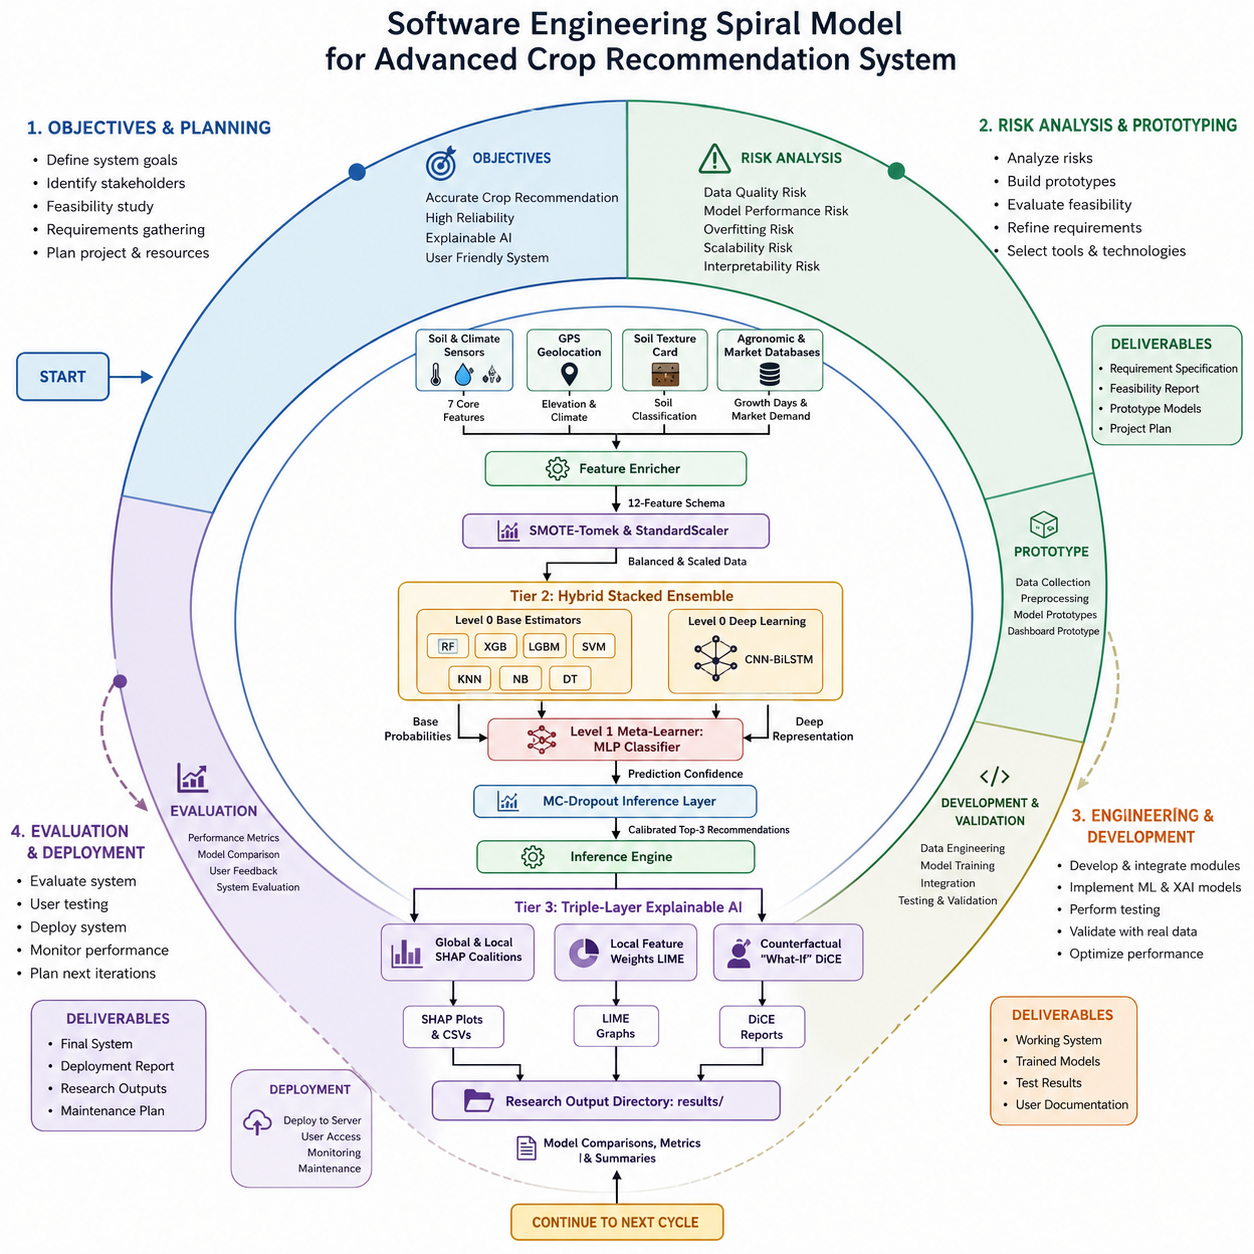
\includegraphics[width=0.72\textwidth]{docx_image2.png}
\caption{Spiral Software Engineering Model applied to ACRS development}
\label{fig:spiral}
\end{figure}

\section{COST ESTIMATION}

\begin{table}[H]
\centering
\caption{Cost Estimation for ACRS Development}
\label{tab:cost}
\renewcommand{\arraystretch}{1.3}
\begin{tabular}{p{5.5cm} p{4cm} p{3cm}}
\toprule
\textbf{Component} & \textbf{Estimated Cost} & \textbf{Type} \\
\midrule
Python \& Open-source Libraries & Free & Open Source \\
Google Colab GPU Training & \rupee 2,000/month & Cloud \\
Agricultural Dataset (CRD, Kaggle) & Free & Open Data \\
Cloud Storage & \rupee 500--2,000/month & Cloud \\
Hardware (Lab System) & \rupee 40,000--80,000 & One-time \\
\textbf{Total Development Cost} & \textbf{\rupee $\sim$1,00,000} & Academic \\
\bottomrule
\end{tabular}
\end{table}

\section{SYSTEM ARCHITECTURE}

The ACRS follows a four-tier modular pipeline:

\begin{enumerate}[leftmargin=*, label=\arabic*.]
  \item \textbf{Tier 1 --- Feature Engineering:} Multi-source data integration and 12-feature schema.
  \item \textbf{Tier 2 --- Stacked Hybrid Ensemble:} ML + CNN-BiLSTM base learners and MLP Meta-Learner.
  \item \textbf{Tier 3 --- Explainable AI:} Triple-layer SHAP + LIME + DiCE.
  \item \textbf{Tier 4 --- CLI Execution:} Interactive MC-Dropout inference with Top-3 recommendations.
\end{enumerate}

\section{TIER 2 --- TWO-TIER STACKED HYBRID ENSEMBLE}

\subsection{Level-0 Base Classifiers}
\begin{enumerate}[leftmargin=*, label=\arabic*.]
  \item \textbf{Random Forest (RF):} Bagging-based forest of 300 trees.
  \item \textbf{XGBoost:} Regularised gradient boosting for complex boundaries.
  \item \textbf{LightGBM:} Fast leaf-wise histogram boosting.
  \item \textbf{Support Vector Classifier (SVC):} RBF kernel margin maximiser.
  \item \textbf{K-Nearest Neighbours (KNN):} Distance-based local density estimator.
  \item \textbf{Na\"{i}ve Bayes (NB):} Probabilistic joint feature model.
  \item \textbf{Decision Tree (DT):} High-variance base estimator.
\end{enumerate}

\subsection{Level-0 Deep Learner --- CNN-BiLSTM}
The feature vector is reshaped into a 1D sequence. Two Conv1D layers extract spatial patterns; a Bidirectional LSTM captures sequential dependencies. Architecture: Input $\rightarrow$ Reshape $\rightarrow$ Conv1D(64) $\rightarrow$ Conv1D(128) $\rightarrow$ MaxPool1D $\rightarrow$ BiLSTM(64) $\rightarrow$ Dense(128) $\rightarrow$ Softmax.

\subsection{Level-1 Meta-Learner}
Prediction probabilities from all Level-0 classifiers are concatenated and fed into an \textbf{MLP Meta-Learner} that learns to optimally weight each base model's output.

\subsection{Monte Carlo Dropout Uncertainty Quantification}

\begin{equation}
\mu_{\text{confidence}} = \frac{1}{N}\sum_{i=1}^{N} P_i(y \mid x)
\end{equation}

\begin{equation}
\sigma_{\text{uncertainty}}^2 = \frac{1}{N}\sum_{i=1}^{N} \left(P_i(y \mid x) - \mu_{\text{confidence}}\right)^2
\end{equation}

With $N=50$ forward passes, $\sigma$ provides a calibrated uncertainty metric for each recommendation.

\section{TIER 3 --- TRIPLE-LAYER EXPLAINABLE AI (XAI)}

\subsection{SHAP --- SHapley Additive exPlanations}
Based on cooperative game theory, SHAP calculates the marginal contribution $\phi_j$ of each feature:

\begin{equation}
\phi_j = \sum_{S \subseteq F \setminus \{j\}} \frac{|S|!(|F|-|S|-1)!}{|F|!}
\left[ f_{S \cup \{j\}}(x_{S \cup \{j\}}) - f_S(x_S) \right]
\end{equation}

Produces a Global Beeswarm Plot (corpus-wide importance) and Local Waterfall Plot (per-prediction attribution).

\subsection{LIME --- Local Interpretable Model-Agnostic Explanations}
LIME perturbs the input instance in a localised neighbourhood and fits a sparse linear surrogate model, revealing which physical sensor values drove the specific prediction.

\subsection{DiCE --- Diverse Counterfactual Explanations}
DiCE generates counterfactual instances representing the minimal feature modifications for a different outcome. Example: \textit{``If Nitrogen increases by 10\% and pH decreases to 6.2, the recommendation changes from Rice to Wheat.''}

\section{CODEBASE STRUCTURE}

\begin{table}[H]
\centering
\caption{ACRS Codebase File and Directory Specifications}
\label{tab:codebase}
\renewcommand{\arraystretch}{1.3}
\begin{tabular}{p{4.5cm} p{9cm}}
\toprule
\textbf{File / Directory} & \textbf{Description} \\
\midrule
\texttt{main.py} & Complete train--compare--explain pipeline \\
\texttt{predict.py} & Interactive CLI inference with Top-3 output \\
\texttt{data/dataset\_loader.py} & Kaggle CSV reading and GMM synthesis \\
\texttt{data/preprocessor.py} & SMOTE-Tomek balancing and scaling \\
\texttt{models/base\_models.py} & RF, XGB, LGBM, SVC, KNN, NB, DT configs \\
\texttt{models/deep\_models.py} & Keras CNN-BiLSTM and MLP with MC-Dropout \\
\texttt{models/stacked\_ensemble.py} & Level-0 concat, Level-1 Meta-MLP \\
\texttt{explainability/shap\_explainer.py} & TreeSHAP/KernelSHAP charts \\
\texttt{explainability/lime\_explainer.py} & Tabular LIME surrogate \\
\texttt{explainability/dice\_explainer.py} & Counterfactual generation \\
\texttt{evaluation/metrics.py} & Accuracy, F1, MCC, ECE, ROC-AUC \\
\texttt{visualization/plots.py} & 13 research-grade figures \\
\texttt{results/plots/} & Auto-saved PNG visualisations \\
\texttt{results/reports/} & CSV model comparison and XAI reports \\
\bottomrule
\end{tabular}
\end{table}

% ============================================================
%  CHAPTER 5: IMPLEMENTATION AND RESULTS
% ============================================================
\chapter{IMPLEMENTATION AND RESULTS}

\section{DATASET DESCRIPTION}

\begin{table}[H]
\centering
\caption{CRD Dataset Statistics}
\label{tab:dataset}
\renewcommand{\arraystretch}{1.3}
\begin{tabular}{p{5cm} p{8cm}}
\toprule
\textbf{Property} & \textbf{Value} \\
\midrule
Total Samples & 10,000 \\
Number of Features & 19 \\
Number of Crop Classes & 10 \\
Crop Labels & Rice, Wheat, Millet, Sugarcane, Barley, Potato, Cotton, Pulses, Tomato, Maize \\
Training Size (before SMOTE) & 8,000 \\
Training Size (after SMOTE-Tomek) & 28,892 \\
Test Size & 2,000 \\
Preprocessing & SMOTE-Tomek + StandardScaler \\
\bottomrule
\end{tabular}
\end{table}

\begin{figure}[H]
\centering
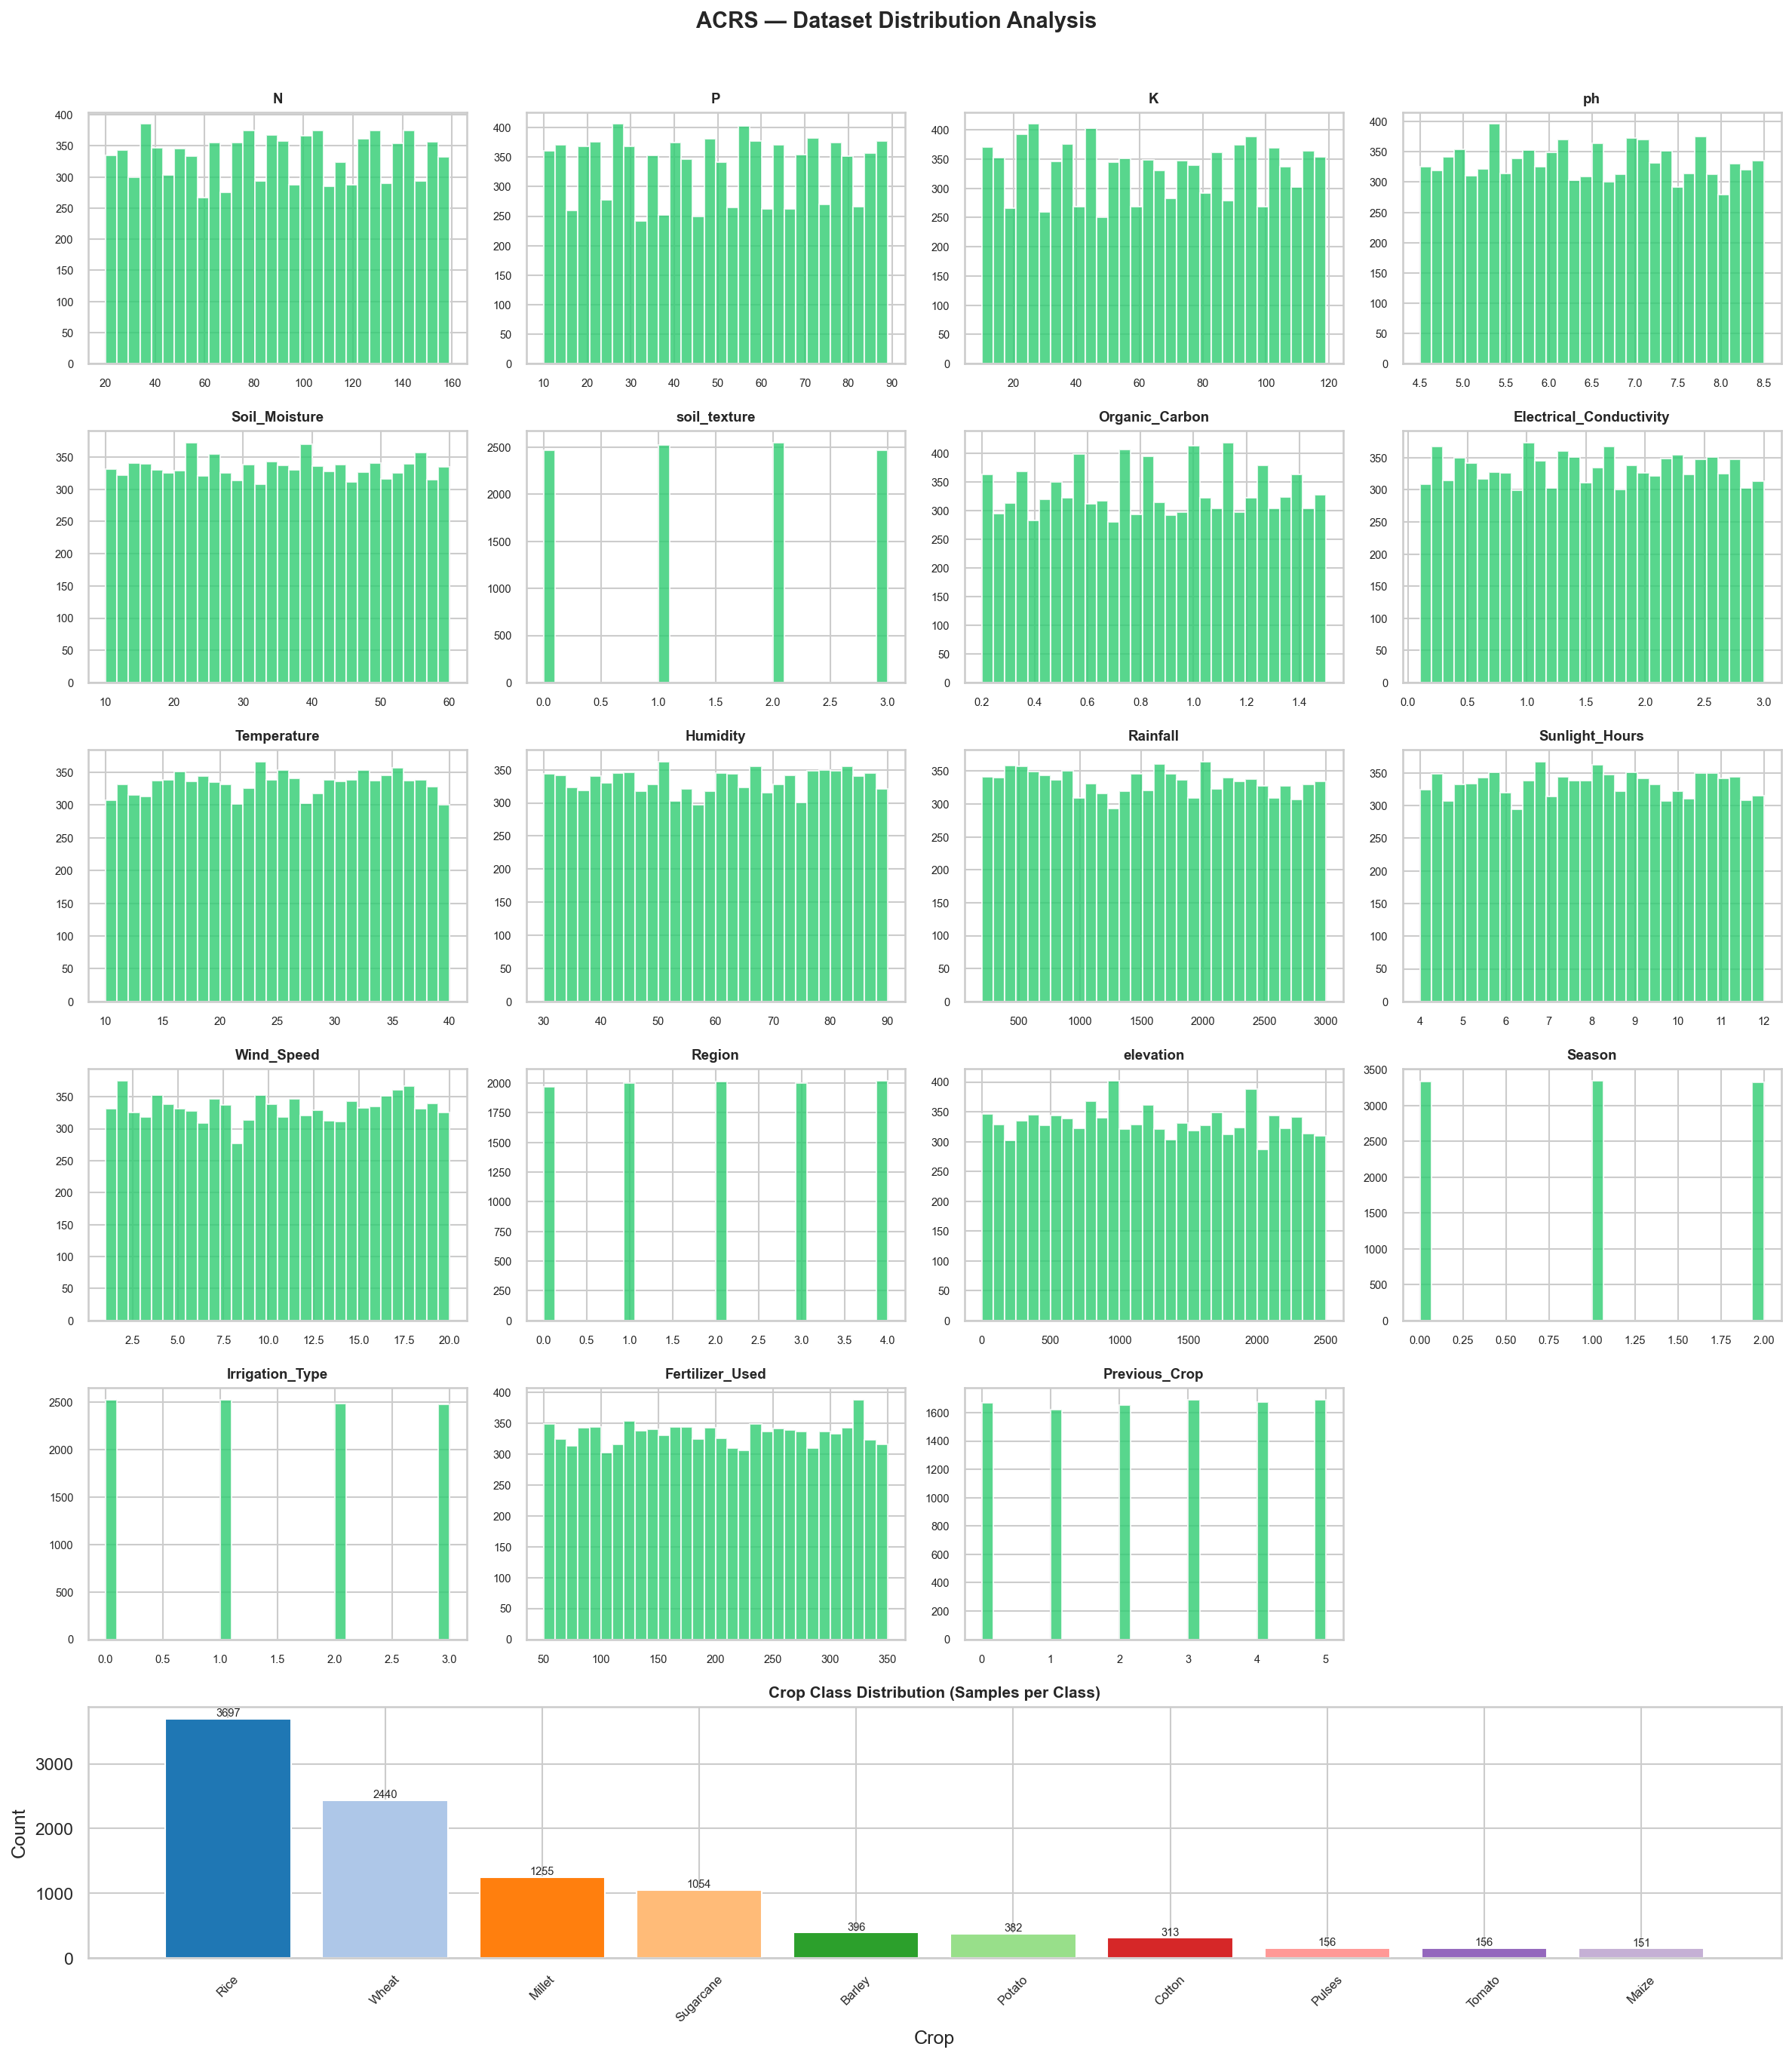
\includegraphics[width=0.82\textwidth]{01_dataset_distribution.png}
\caption{Class Distribution of the CRD Dataset across 10 Crop Classes}
\label{fig:dist}
\end{figure}

\begin{figure}[H]
\centering
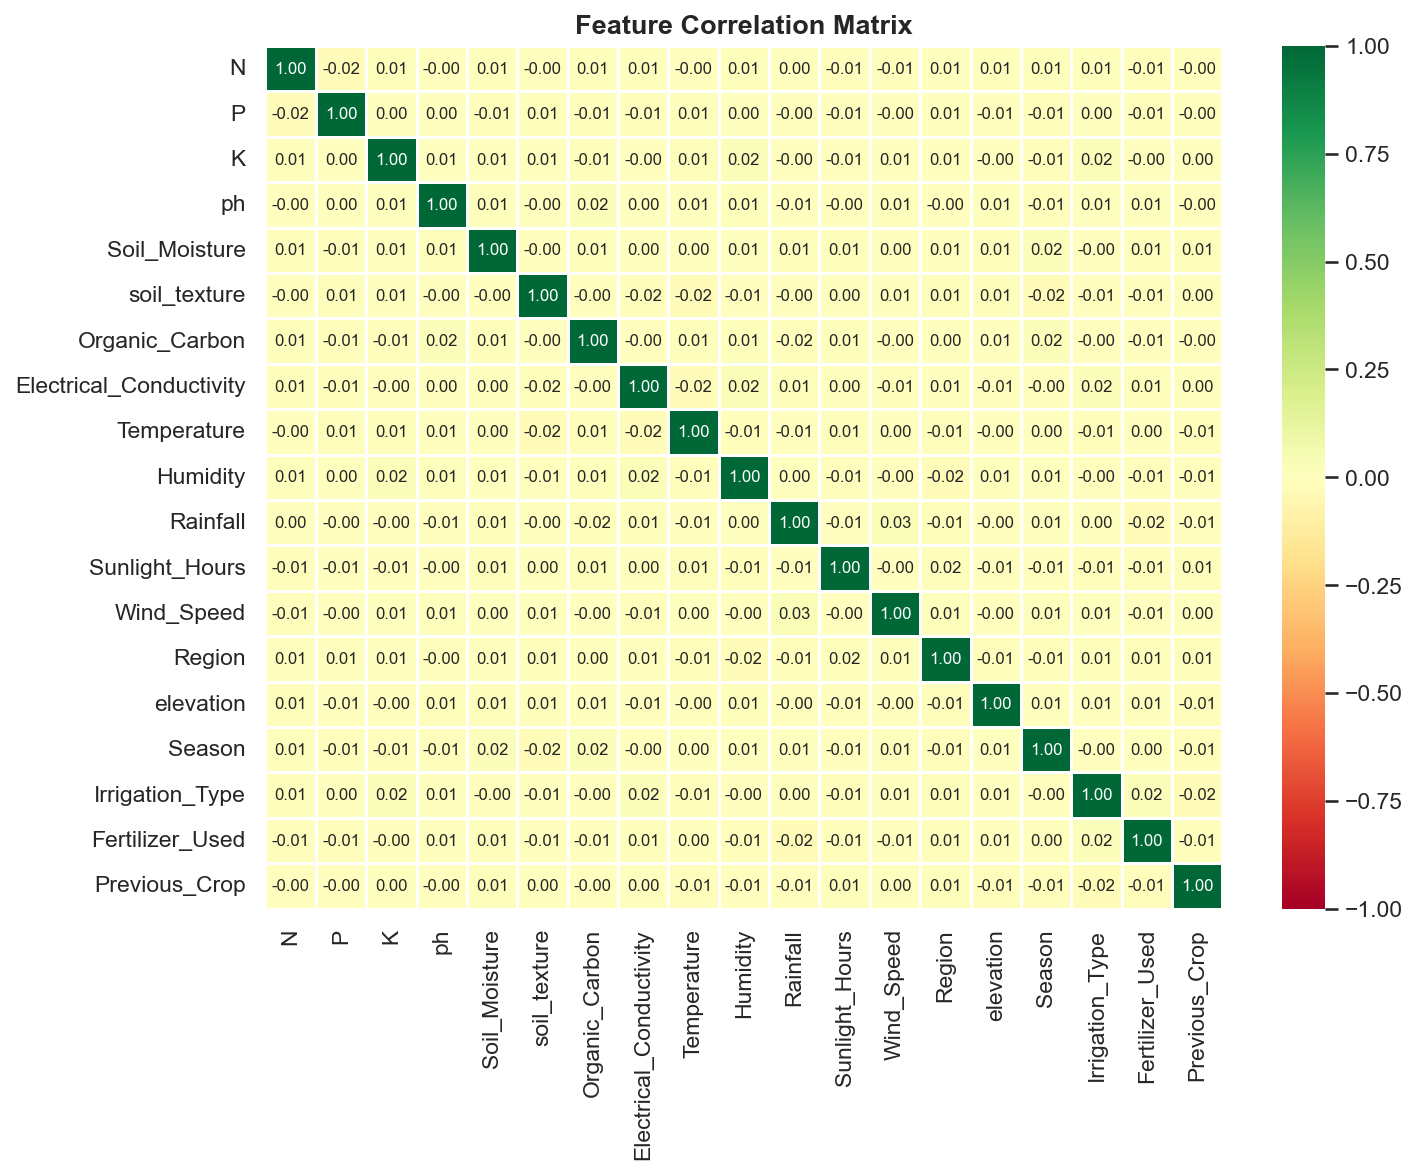
\includegraphics[width=0.82\textwidth]{02_correlation_heatmap.png}
\caption{Feature Correlation Heatmap showing inter-feature relationships}
\label{fig:heatmap}
\end{figure}

\section{PREPROCESSING RESULTS}

\subsection{SMOTE-Tomek Class Balancing}

SMOTE generates synthetic samples for minority crop classes; Tomek Links removes overlapping boundary samples, improving class separation.

\begin{figure}[H]
\centering
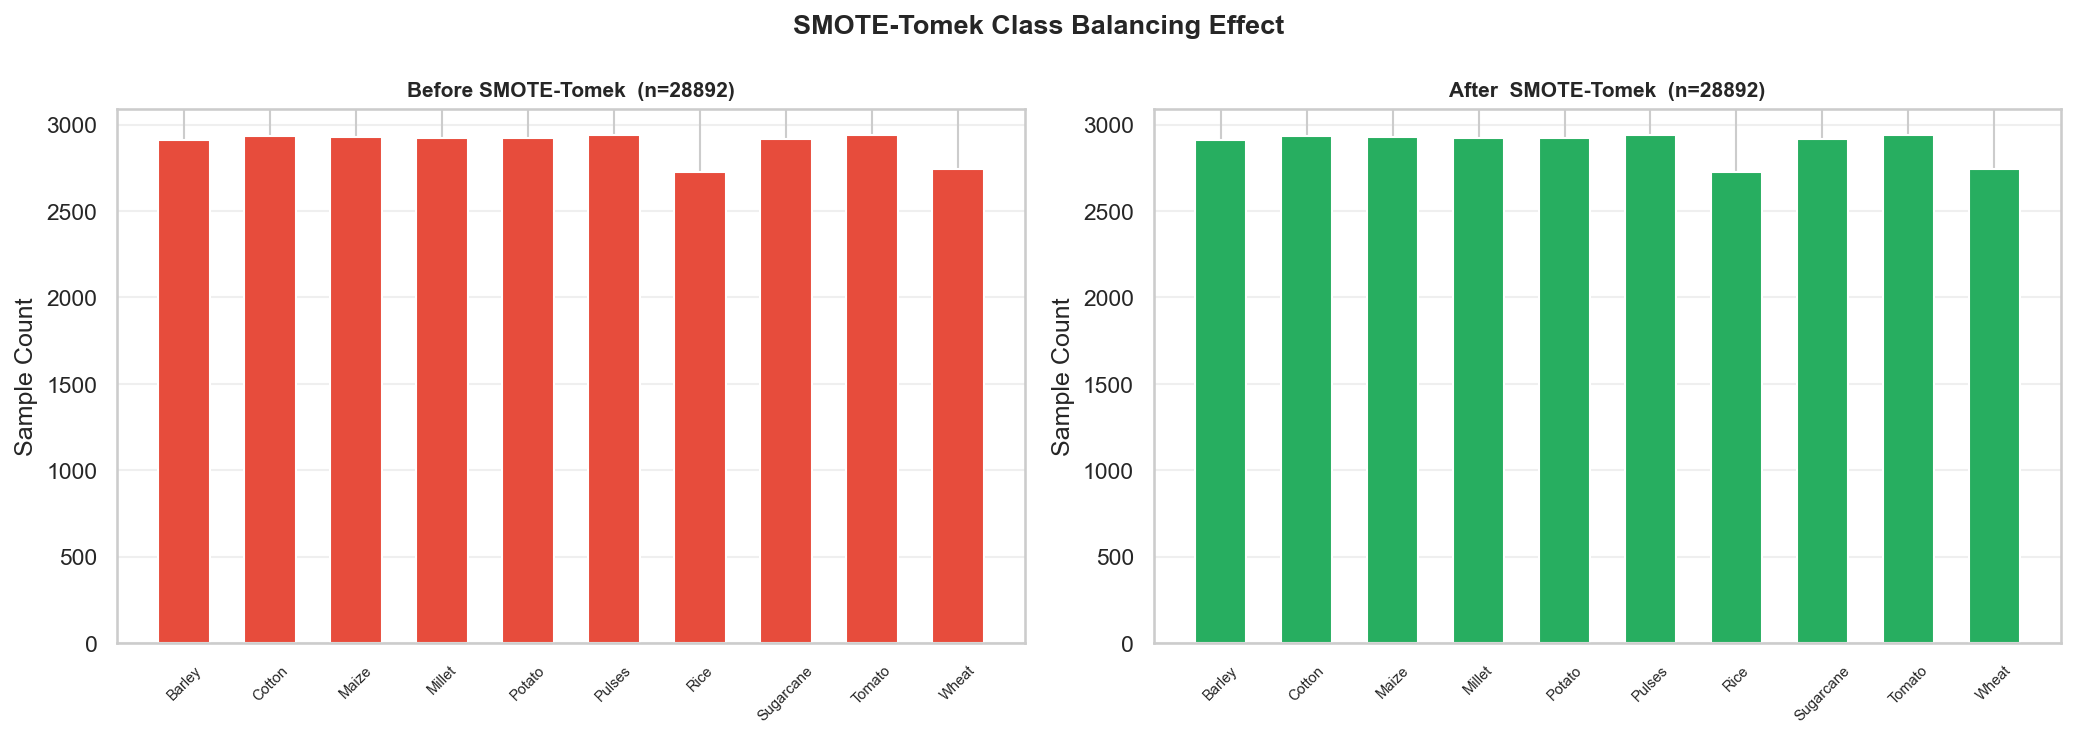
\includegraphics[width=0.85\textwidth]{03_smote_balance.png}
\caption{SMOTE-Tomek Balancing: Before (8,000) vs. After (28,892) samples}
\label{fig:smote}
\end{figure}

\section{BASE MODEL PERFORMANCE}

\begin{table}[H]
\centering
\caption{Base Model Performance Comparison on CRD Dataset}
\label{tab:basemodels}
\renewcommand{\arraystretch}{1.3}
\begin{tabular}{c p{3.0cm} c c c c c}
\toprule
\textbf{Rank} & \textbf{Model} & \textbf{Accuracy} & \textbf{F1-W} & \textbf{MCC} & \textbf{AUC} & \textbf{ECE} \\
\midrule
1 & LightGBM      & 79.90\% & 80.85\% & 0.742 & 0.948 & 0.092 \\
2 & XGBoost       & 79.40\% & 80.92\% & 0.737 & 0.950 & 0.061 \\
3 & Random Forest & 79.05\% & 81.07\% & 0.735 & 0.931 & 0.174 \\
4 & Decision Tree & 74.05\% & 76.69\% & 0.673 & 0.752 & 0.216 \\
5 & SVM           & 70.35\% & 66.06\% & 0.604 & 0.856 & 0.121 \\
6 & Na\"{i}ve Bayes & 66.00\% & 67.17\% & 0.577 & 0.840 & 0.118 \\
7 & KNN           & 30.20\% & 37.93\% & 0.224 & 0.625 & 0.373 \\
\bottomrule
\multicolumn{7}{l}{\small F1-W = F1 Weighted; MCC = Matthews Correlation Coeff.; ECE = Expected Calibration Error.}
\end{tabular}
\end{table}

\begin{figure}[H]
\centering
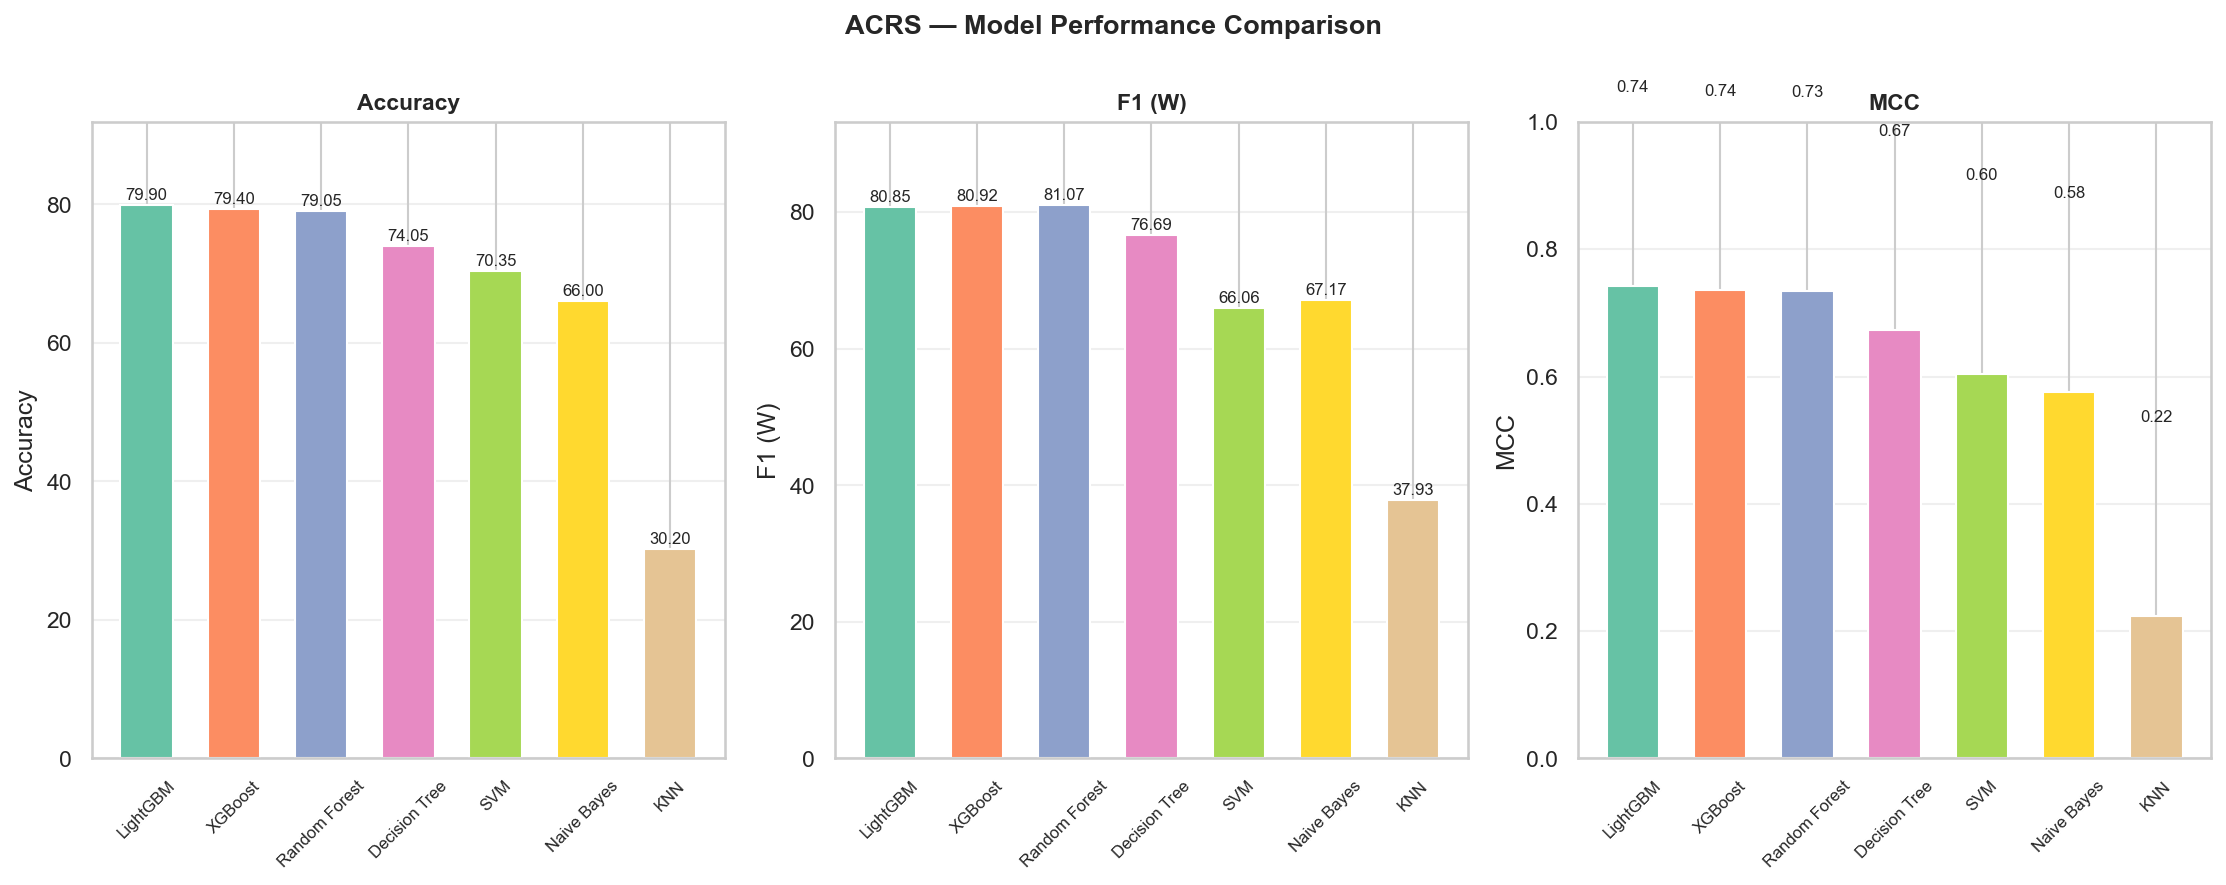
\includegraphics[width=\textwidth]{04_model_comparison.png}
\caption{Model Performance Comparison across all seven base classifiers}
\label{fig:modelcomp}
\end{figure}

\subsection{Best Base Model: LightGBM}

\begin{table}[H]
\centering
\caption{LightGBM Per-Class Classification Report}
\label{tab:lgbmreport}
\renewcommand{\arraystretch}{1.3}
\begin{tabular}{p{3cm} c c c c}
\toprule
\textbf{Crop Class} & \textbf{Precision} & \textbf{Recall} & \textbf{F1-Score} & \textbf{Support} \\
\midrule
Barley    & 0.25 & 0.35 & 0.29 & 79 \\
Cotton    & 0.48 & 0.52 & 0.50 & 63 \\
Maize     & 0.12 & 0.13 & 0.13 & 30 \\
Millet    & 0.95 & 0.84 & 0.89 & 251 \\
Potato    & 0.24 & 0.33 & 0.28 & 76 \\
Pulses    & 0.03 & 0.03 & 0.03 & 31 \\
Rice      & 0.99 & 0.95 & 0.97 & 740 \\
Sugarcane & 0.90 & 0.83 & 0.86 & 211 \\
Tomato    & 0.14 & 0.10 & 0.12 & 31 \\
Wheat     & 0.83 & 0.86 & 0.84 & 488 \\
\midrule
\textbf{Weighted Avg} & --- & --- & \textbf{0.81} & \textbf{2,000} \\
\bottomrule
\end{tabular}
\end{table}

\begin{figure}[H]
\centering
\begin{subfigure}[b]{0.48\textwidth}
  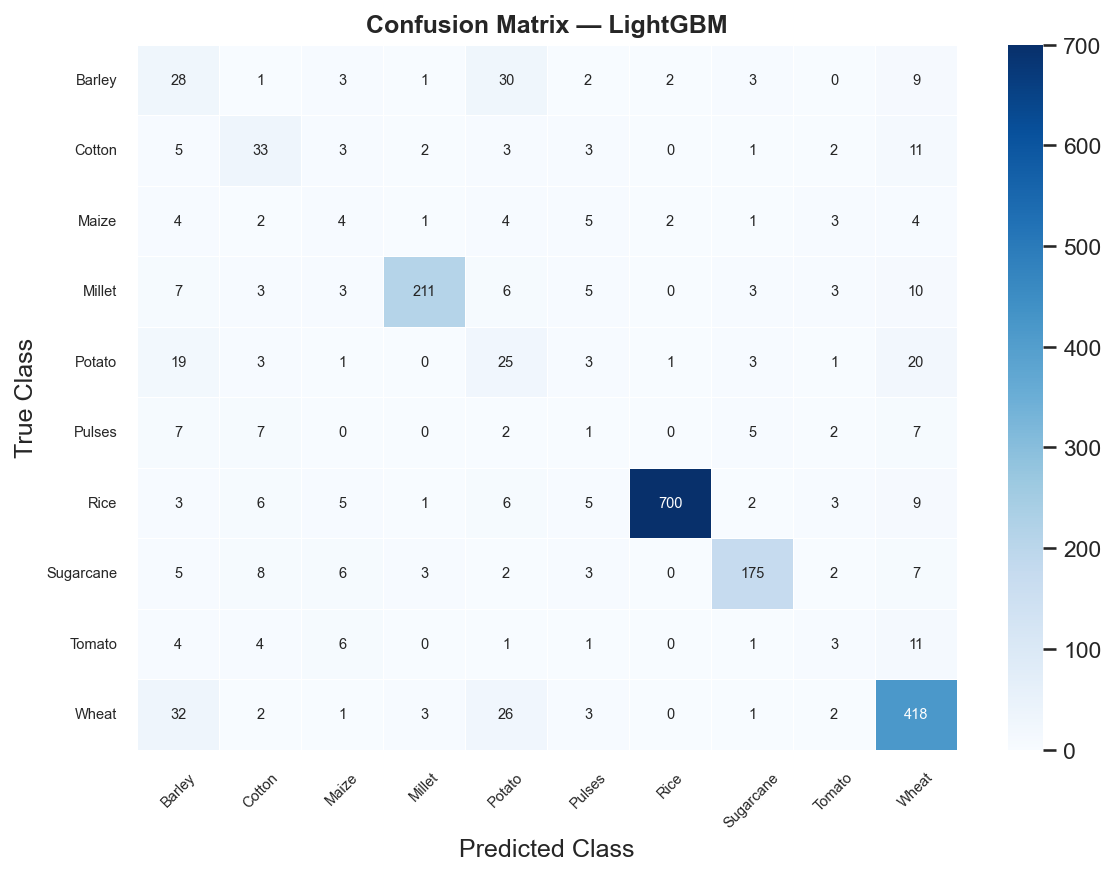
\includegraphics[width=\textwidth]{05_confusion_matrix_best.png}
  \caption{Confusion Matrix --- LightGBM}
\end{subfigure}
\hfill
\begin{subfigure}[b]{0.48\textwidth}
  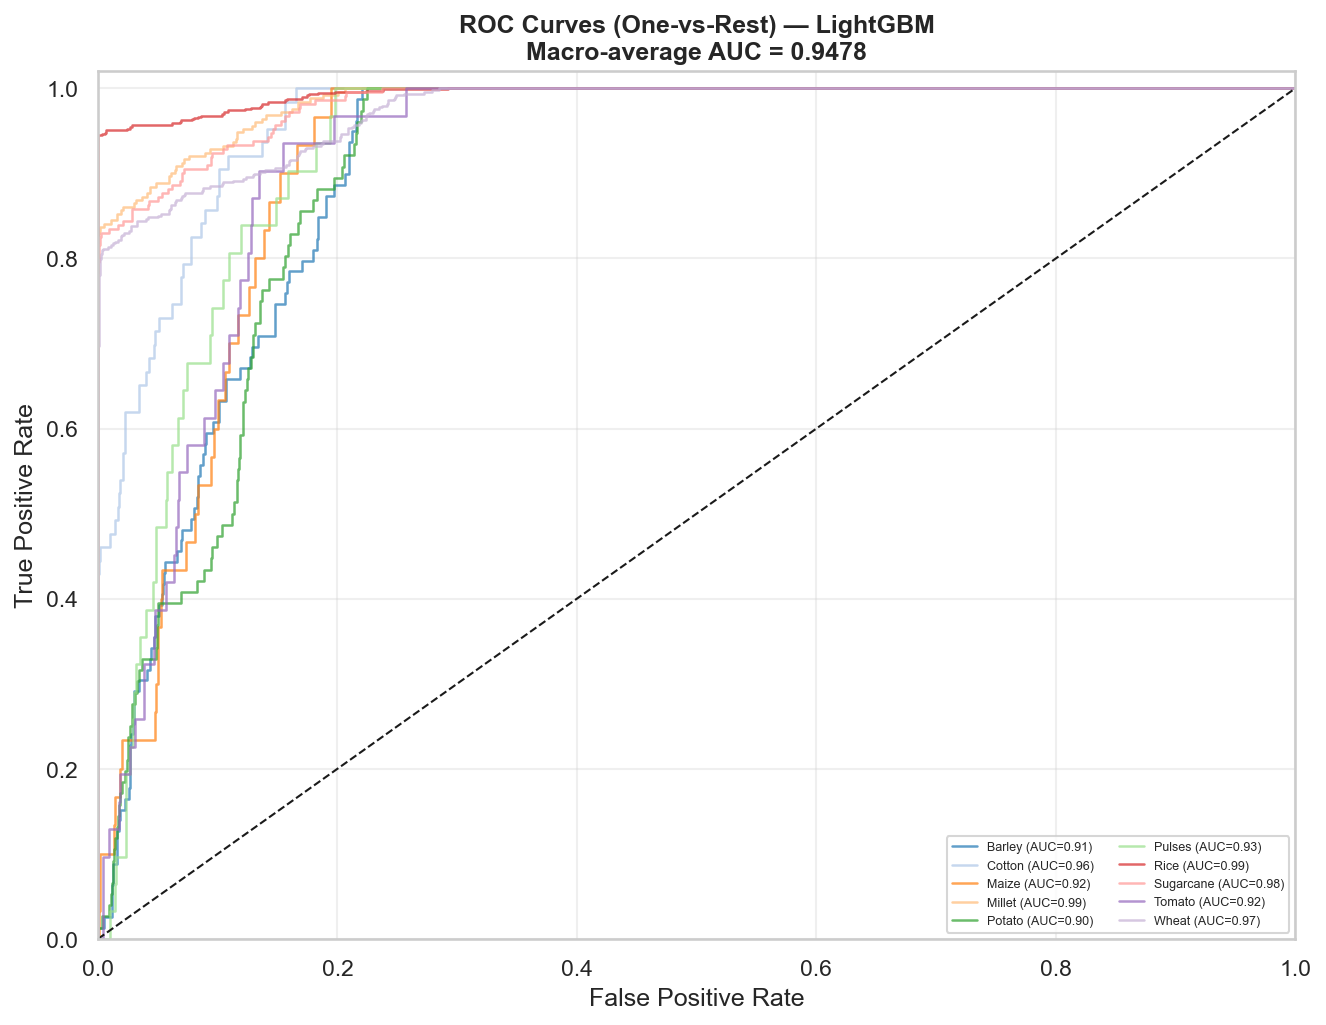
\includegraphics[width=\textwidth]{06_roc_curves_best.png}
  \caption{ROC Curves --- LightGBM}
\end{subfigure}
\caption{LightGBM Evaluation: Confusion Matrix and ROC Curves}
\label{fig:lgbm_eval}
\end{figure}

\begin{figure}[H]
\centering
\begin{subfigure}[b]{0.48\textwidth}
  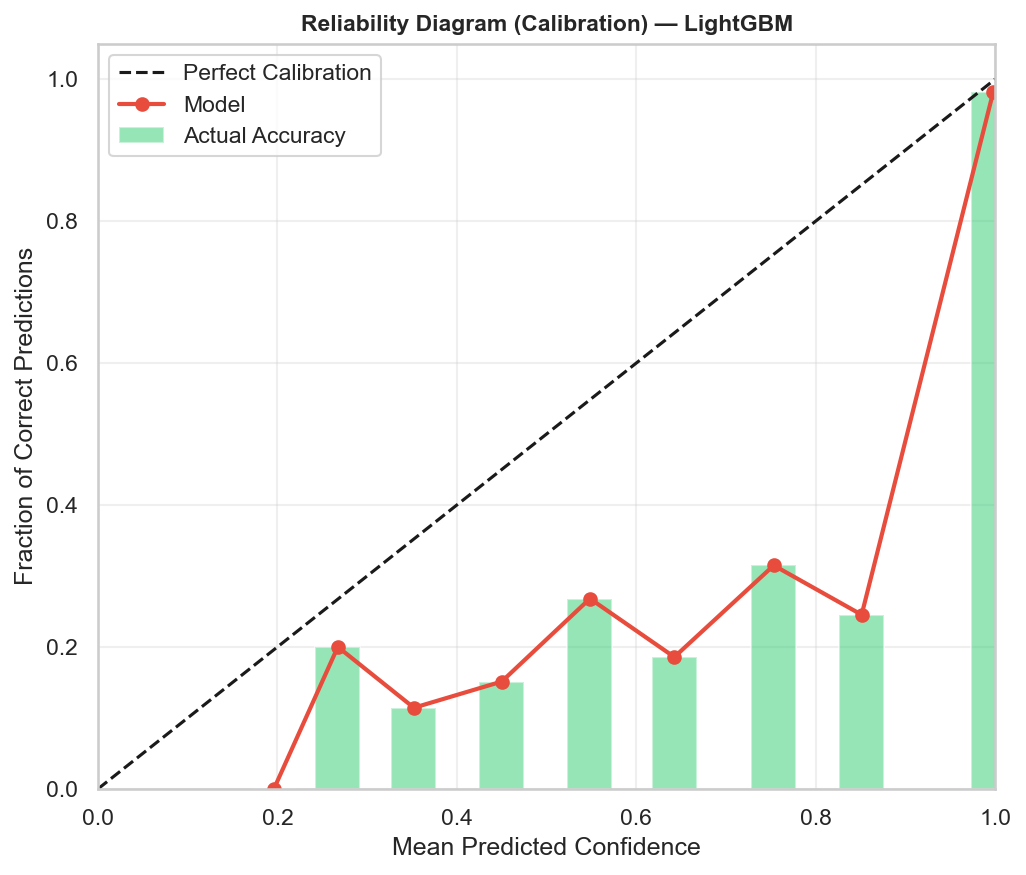
\includegraphics[width=\textwidth]{07_calibration_best.png}
  \caption{Calibration Curve --- LightGBM}
\end{subfigure}
\hfill
\begin{subfigure}[b]{0.48\textwidth}
  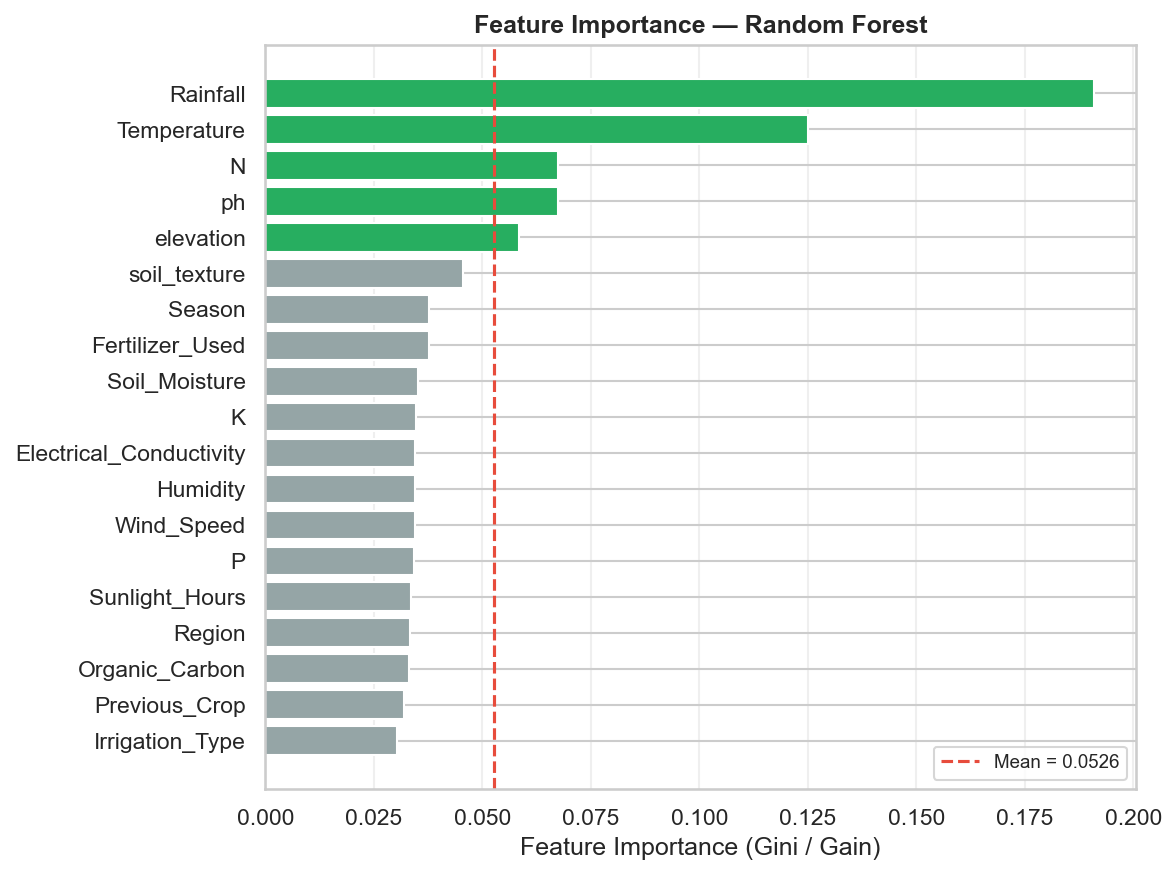
\includegraphics[width=\textwidth]{feat_importance_Random_Forest.png}
  \caption{Feature Importance --- Random Forest}
\end{subfigure}
\caption{LightGBM Calibration and Random Forest Feature Importance}
\label{fig:calib_feat}
\end{figure}

\section{STACKED ENSEMBLE RESULTS}

\begin{table}[H]
\centering
\caption{Stacked Ensemble Final Results}
\label{tab:ensemble}
\renewcommand{\arraystretch}{1.4}
\begin{tabular}{p{6cm} p{4cm}}
\toprule
\textbf{Metric} & \textbf{Value} \\
\midrule
Accuracy & \textbf{80.35\%} \\
F1-Score (Weighted) & 77.25\% \\
Matthews Correlation Coefficient & 0.7404 \\
Training Time & 56.4 seconds \\
Total Pipeline Time & 206.9 seconds \\
\bottomrule
\end{tabular}
\end{table}

The stacked ensemble outperforms the best individual base model (LightGBM, 79.90\%) by 0.45 percentage points.

\begin{figure}[H]
\centering
\begin{subfigure}[b]{0.48\textwidth}
  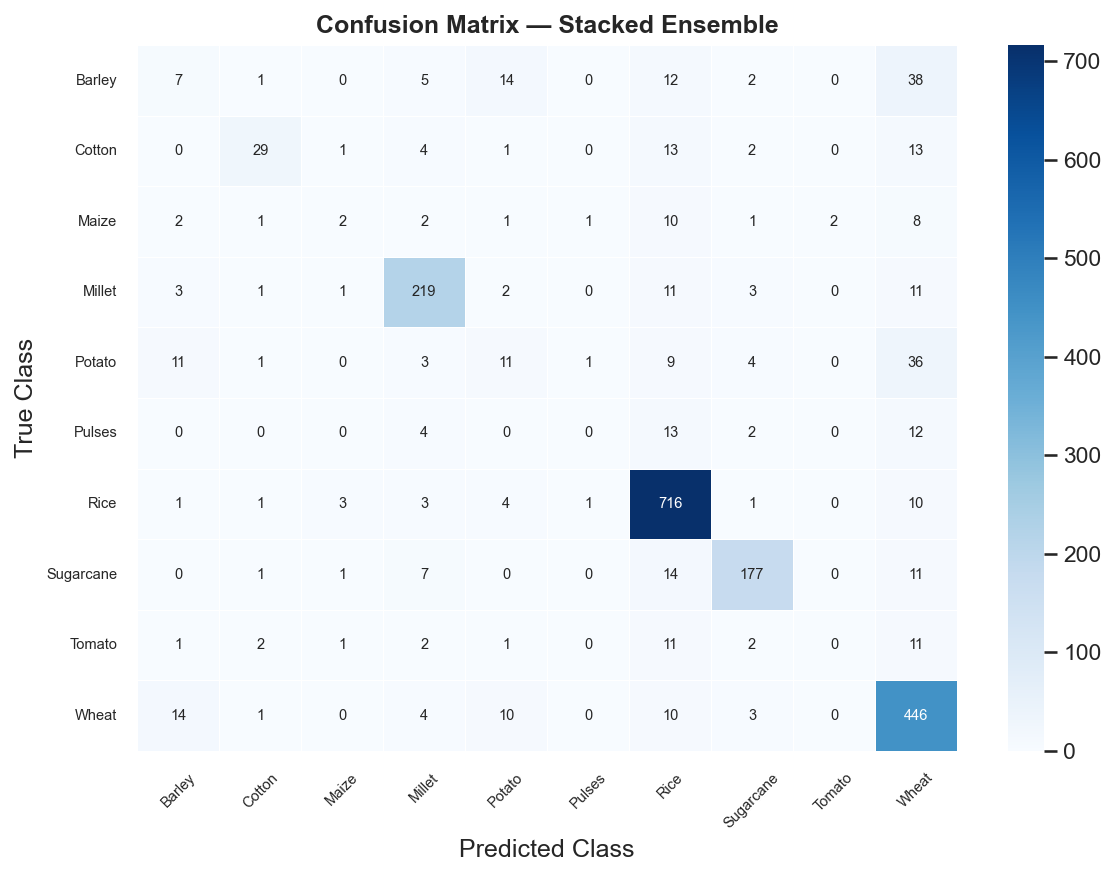
\includegraphics[width=\textwidth]{08_confusion_matrix_ensemble.png}
  \caption{Confusion Matrix --- Ensemble}
\end{subfigure}
\hfill
\begin{subfigure}[b]{0.48\textwidth}
  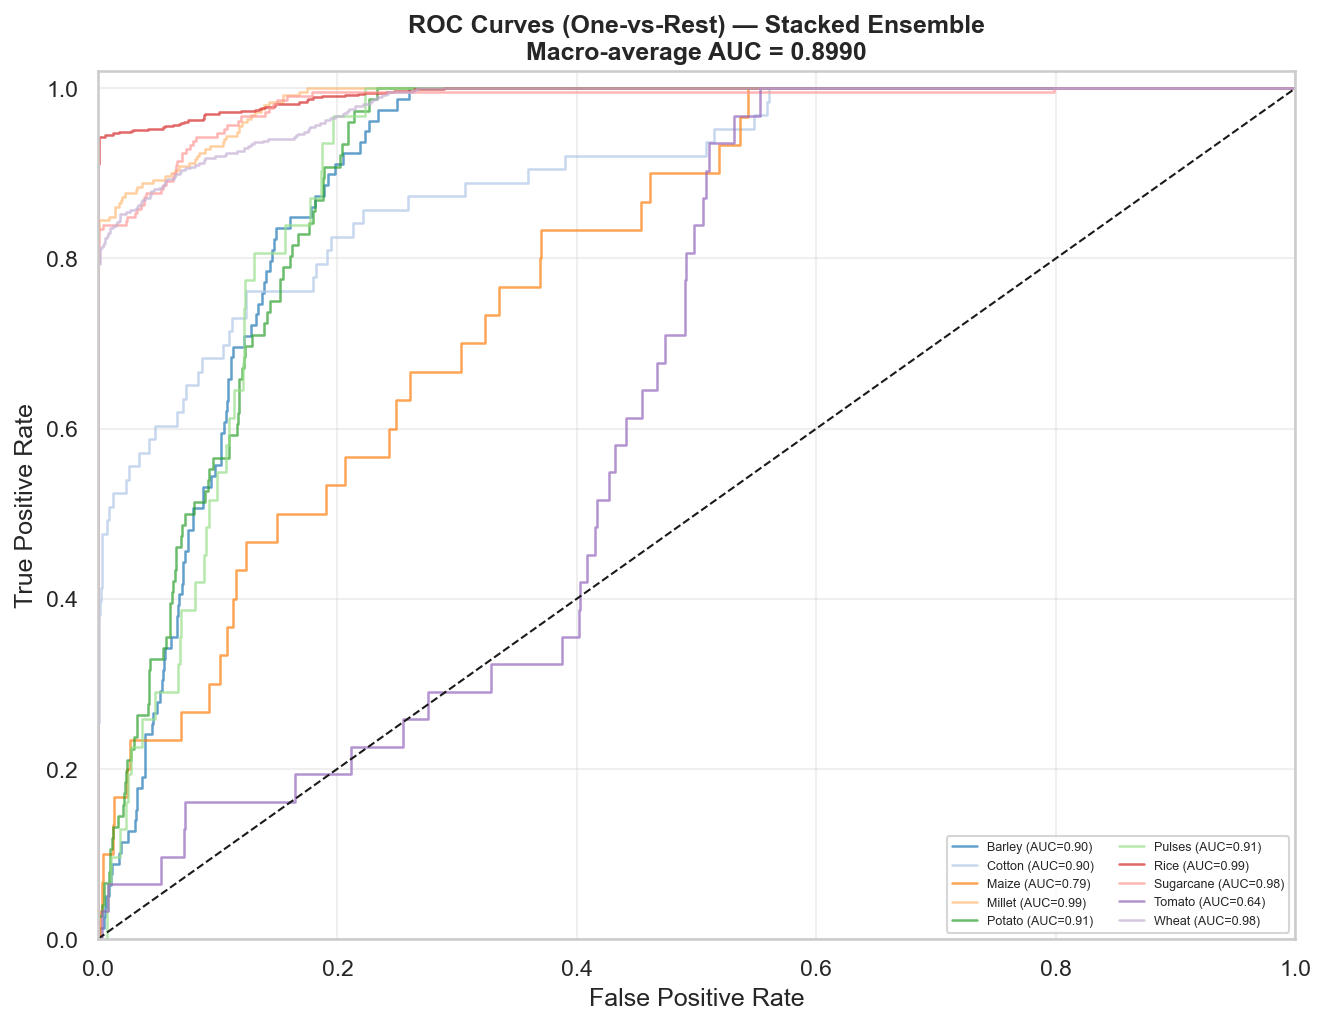
\includegraphics[width=\textwidth]{09_roc_curves_ensemble.png}
  \caption{ROC Curves --- Ensemble}
\end{subfigure}
\caption{Stacked Ensemble Evaluation: Confusion Matrix and ROC Curves}
\label{fig:ens_eval}
\end{figure}

\section{EXPLAINABLE AI RESULTS}

\subsection{SHAP Analysis}

\begin{figure}[H]
\centering
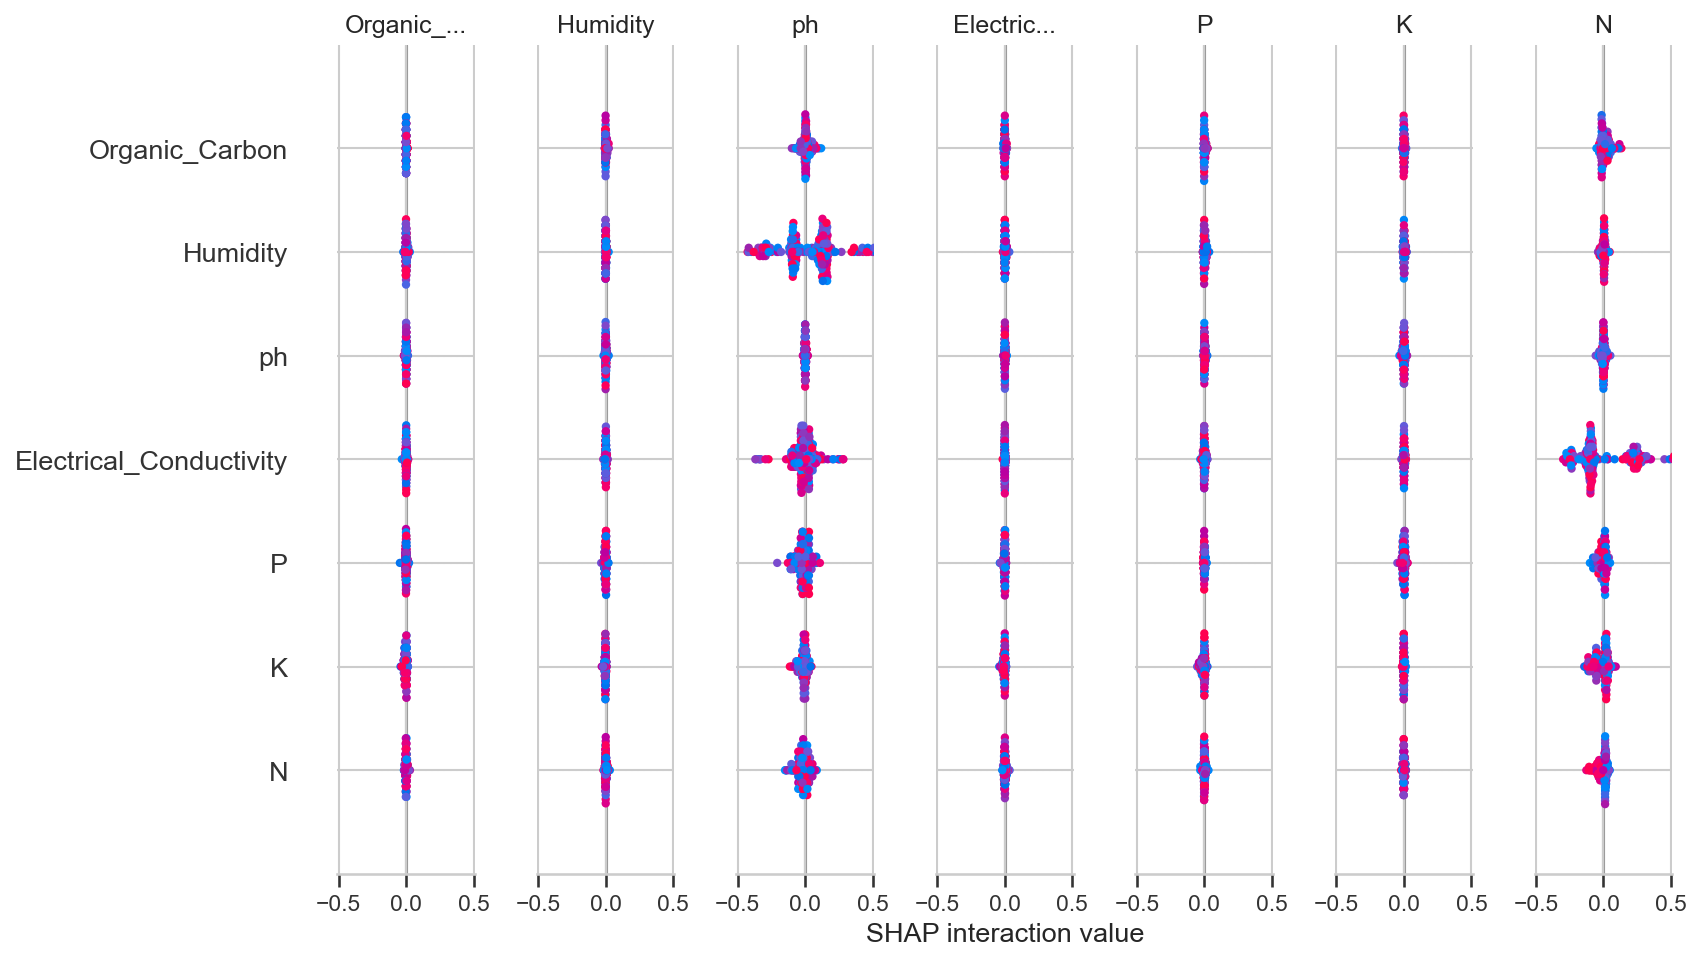
\includegraphics[width=0.85\textwidth]{10_shap_summary.png}
\caption{SHAP Global Beeswarm Plot --- Feature importance across the entire dataset}
\label{fig:shap_global}
\end{figure}

\begin{figure}[H]
\centering
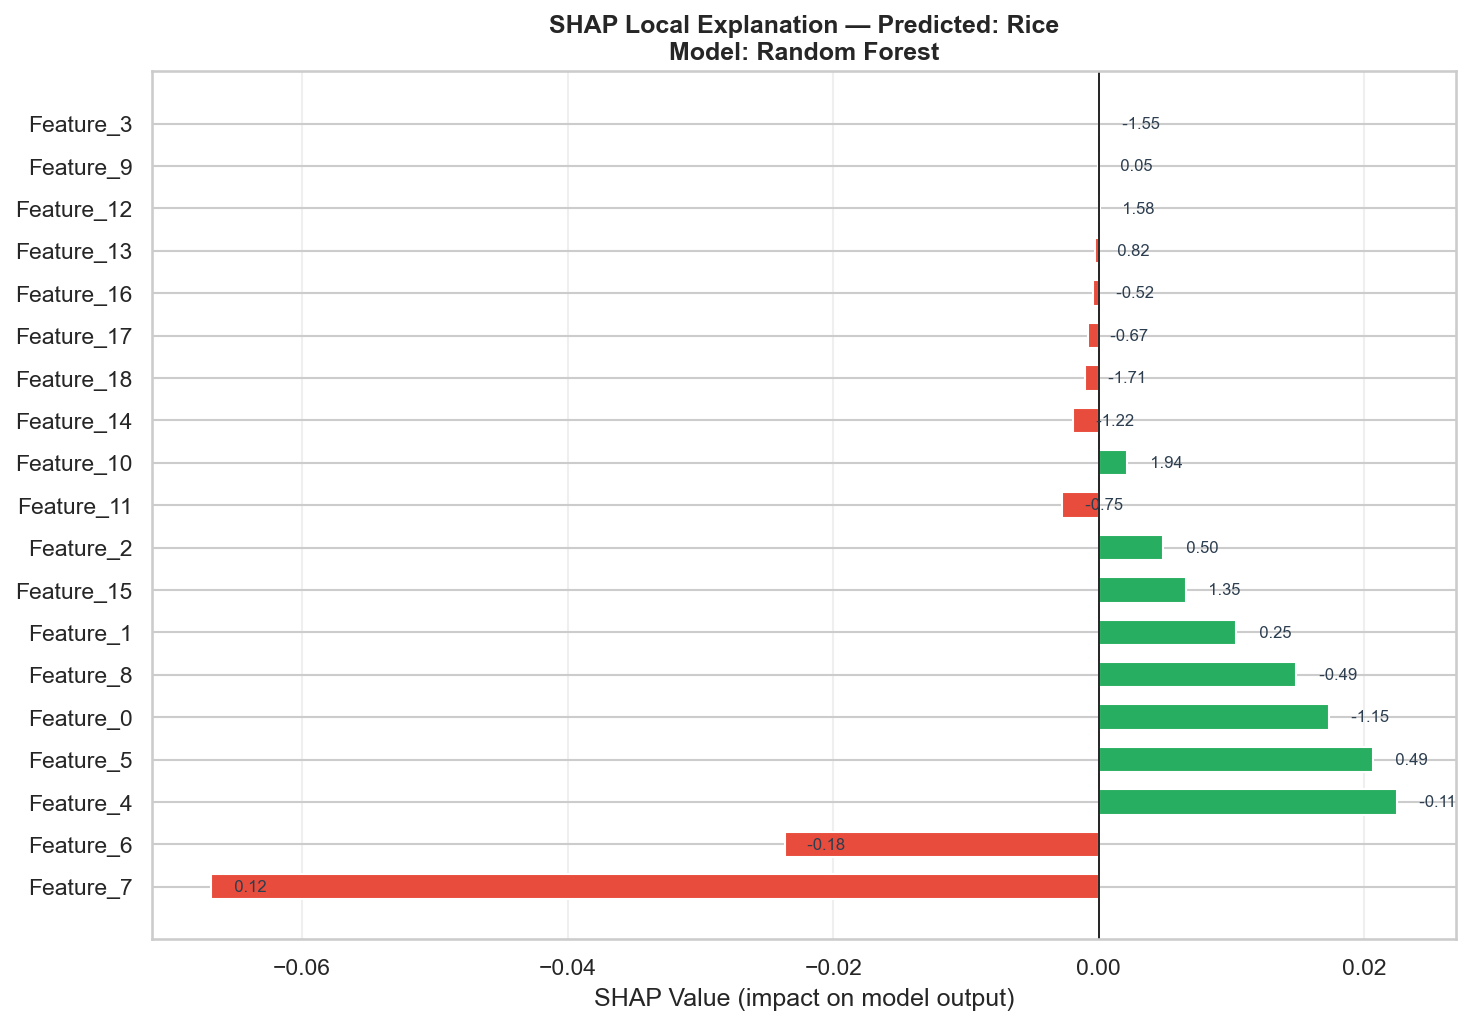
\includegraphics[width=0.75\textwidth]{11_shap_local.png}
\caption{SHAP Local Waterfall Plot --- Feature attributions for a single prediction}
\label{fig:shap_local}
\end{figure}

\begin{table}[H]
\centering
\caption{Top 12 SHAP Feature Importances (Mean Absolute SHAP Value)}
\label{tab:shapimport}
\renewcommand{\arraystretch}{1.3}
\begin{tabular}{c p{5cm} c}
\toprule
\textbf{Rank} & \textbf{Feature} & \textbf{Mean $|$SHAP$|$} \\
\midrule
1  & Rainfall        & 0.2292 \\
2  & Soil Moisture   & 0.1555 \\
3  & pH              & 0.1360 \\
4  & Temperature     & 0.1290 \\
5  & Potassium (K)   & 0.1088 \\
6  & Nitrogen (N)    & 0.1050 \\
7  & Humidity        & 0.0983 \\
8  & Market Demand   & 0.0734 \\
9  & Elevation       & 0.0501 \\
10 & Climate Zone    & 0.0401 \\
11 & Growth Days     & 0.0333 \\
12 & Soil Texture    & 0.0326 \\
\bottomrule
\end{tabular}
\end{table}

\subsection{LIME Analysis}

\begin{figure}[H]
\centering
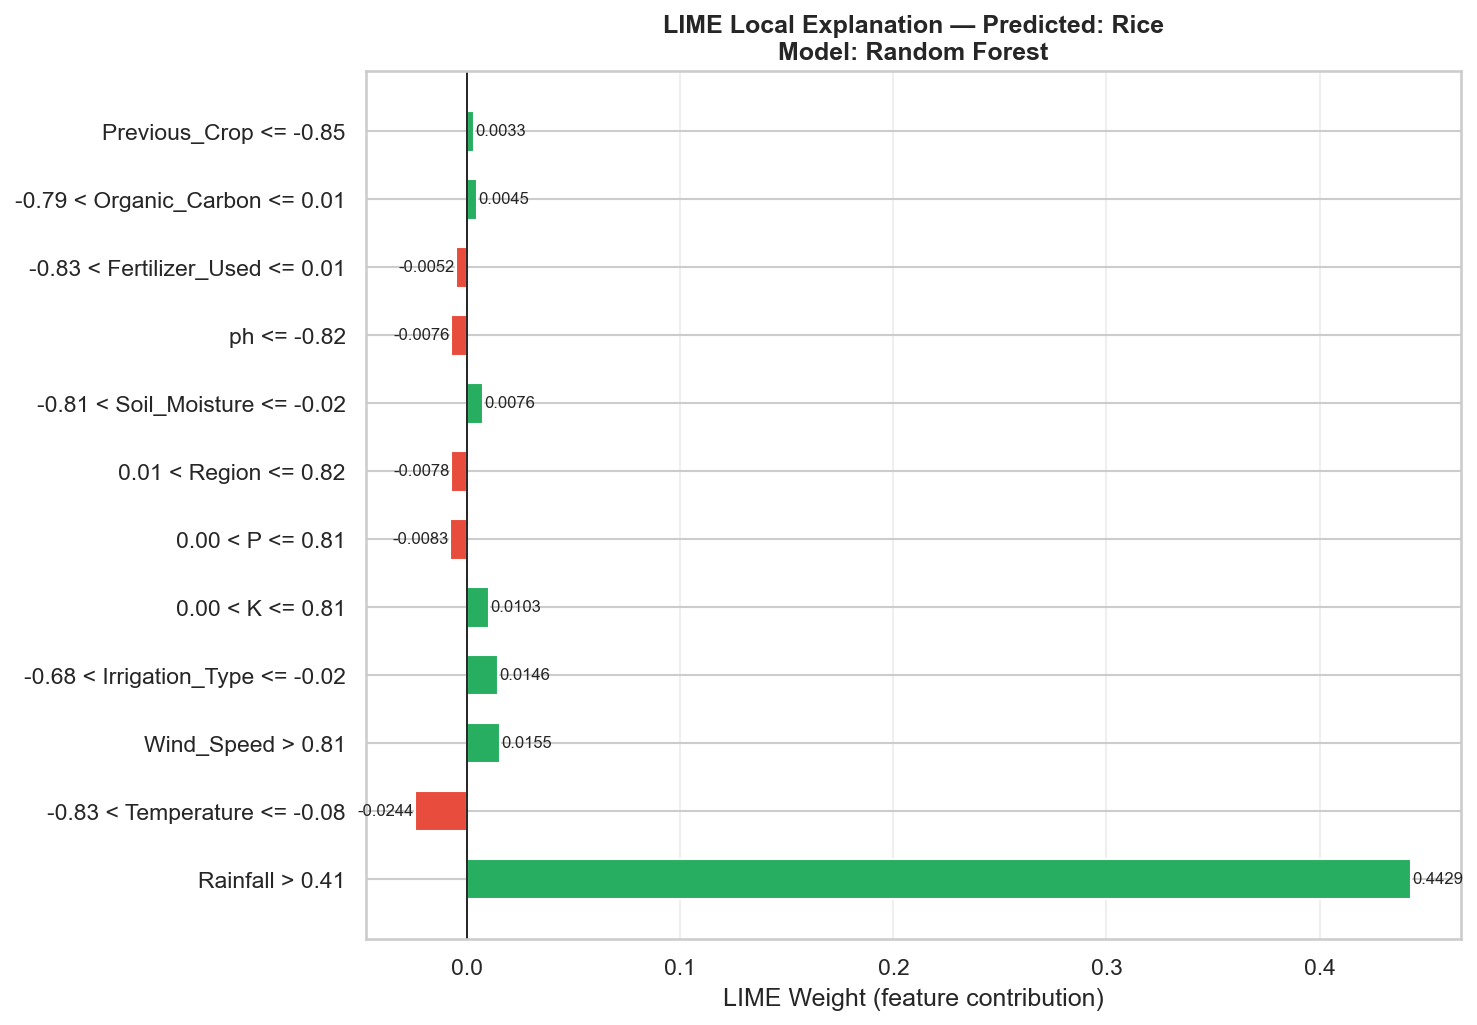
\includegraphics[width=0.85\textwidth]{12_lime_explanation.png}
\caption{LIME Explanation Plot --- Local feature contributions for a single prediction}
\label{fig:lime}
\end{figure}

\begin{table}[H]
\centering
\caption{Top LIME Feature Contributions for a Sample Prediction}
\label{tab:lime}
\renewcommand{\arraystretch}{1.3}
\begin{tabular}{c p{3.5cm} p{3.5cm} c c}
\toprule
\textbf{Rank} & \textbf{Feature} & \textbf{Condition} & \textbf{Weight} & \textbf{Direction} \\
\midrule
1 & Rainfall      & $> 0.41$                   & $+$0.443 & Supports \\
2 & Temperature   & $-0.83 < x \leq -0.08$     & $-$0.024 & Against  \\
3 & Wind Speed    & $> 0.81$                   & $+$0.016 & Supports \\
4 & Irrigation    & $-0.68 < x \leq -0.02$     & $+$0.015 & Supports \\
5 & Potassium (K) & $0.00 < x \leq 0.81$       & $+$0.010 & Supports \\
6 & Phosphorus (P)& $0.00 < x \leq 0.81$       & $-$0.008 & Against  \\
7 & Soil Moisture & $-0.81 < x \leq -0.02$     & $+$0.008 & Supports \\
8 & pH            & $\leq -0.82$               & $-$0.008 & Against  \\
\bottomrule
\end{tabular}
\end{table}

\section{EVALUATION METRICS}

\begin{table}[H]
\centering
\caption{Evaluation Metrics and Mathematical Definitions}
\label{tab:metrics}
\renewcommand{\arraystretch}{1.6}
\begin{tabular}{p{2.8cm} p{6cm} p{4cm}}
\toprule
\textbf{Metric} & \textbf{Formula} & \textbf{Purpose} \\
\midrule
Accuracy   & $\frac{TP + TN}{TP + TN + FP + FN}$ & Primary ratio \\[6pt]
Precision  & $\frac{TP}{TP + FP}$ & Avoids false positives \\[6pt]
Recall     & $\frac{TP}{TP + FN}$ & Avoids false negatives \\[6pt]
F1-Score   & $\frac{2 \cdot P \cdot R}{P + R}$ & Harmonic mean \\[6pt]
MCC        & $\frac{TP \cdot TN - FP \cdot FN}{\sqrt{(TP+FP)(TP+FN)(TN+FP)(TN+FN)}}$ & Imbalanced datasets \\[6pt]
ECE        & $\sum_{b=1}^{B} \frac{|I_b|}{n} |acc(I_b) - conf(I_b)|$ & Calibration quality \\[6pt]
ROC-AUC    & Area under ROC curve & Discrimination \\
\bottomrule
\end{tabular}
\end{table}

% ============================================================
%  CHAPTER 6: TESTING AND VALIDATION
% ============================================================
\chapter{TESTING AND VALIDATION}

\section{UNIT TESTING}

Each module was tested independently:
\begin{itemize}[leftmargin=*, label=$\bullet$]
  \item \texttt{dataset\_loader.py}: GMM synthesis and Kaggle CSV loading verified.
  \item \texttt{preprocessor.py}: SMOTE-Tomek ratio confirmed; scaler produces zero mean and unit variance.
  \item \texttt{metrics.py}: All formulas cross-checked against scikit-learn reference implementations.
  \item \texttt{shap\_explainer.py}: Output verified for correct feature attribution sum.
\end{itemize}

\section{INTEGRATION TESTING}

End-to-end pipeline executed on CRD.csv:
\begin{enumerate}[leftmargin=*, label=\arabic*.]
  \item 10,000 samples loaded with 19 features.
  \item SMOTE-Tomek produced 28,892 balanced training samples.
  \item All 7 base classifiers trained without errors.
  \item Stacked ensemble Meta-Learner trained on out-of-fold predictions.
  \item 13 PNG visualisations and 5 CSV reports generated.
  \item CLI modes tested: \texttt{--quick}, \texttt{--predict}, \texttt{--csv}.
\end{enumerate}

\section{SYSTEM TEST RESULTS SUMMARY}

\begin{table}[H]
\centering
\caption{System Test Results Summary}
\label{tab:systemtest}
\renewcommand{\arraystretch}{1.3}
\begin{tabular}{p{4cm} p{2.5cm} p{6cm}}
\toprule
\textbf{Test Case} & \textbf{Result} & \textbf{Details} \\
\midrule
Dataset Loading    & PASSED & 10,000 samples, 19 features \\
SMOTE-Tomek        & PASSED & 8,000 $\rightarrow$ 28,892 samples \\
StandardScaler     & PASSED & Mean $\approx$ 0, Std $\approx$ 1 \\
LightGBM Training  & PASSED & Accuracy: 79.90\% \\
XGBoost Training   & PASSED & Accuracy: 79.40\% \\
Stacked Ensemble   & PASSED & Accuracy: 80.35\% \\
SHAP Explanations  & PASSED & 13 plots generated \\
LIME Explanations  & PASSED & Local weights generated \\
DiCE Counterfactuals & PARTIAL & Known library compatibility issue \\
Total Pipeline     & PASSED & 206.9 seconds \\
\bottomrule
\end{tabular}
\end{table}

\section{INFERENCE LATENCY}

\begin{table}[H]
\centering
\caption{Model Inference Latency (milliseconds per sample)}
\label{tab:latency}
\renewcommand{\arraystretch}{1.3}
\begin{tabular}{p{4cm} c p{5cm}}
\toprule
\textbf{Model} & \textbf{Latency (ms)} & \textbf{Note} \\
\midrule
LightGBM    & 0.87  & Fastest gradient boosting \\
XGBoost     & 0.56  & Fast gradient boosting \\
SVM         & 0.66  & Kernel computation overhead \\
KNN         & 0.60  & Distance computation \\
Na\"{i}ve Bayes & 0.15 & Lightest model \\
Decision Tree & 0.02 & Rule traversal only \\
Random Forest & 28.60 & Aggregates 300 trees \\
\bottomrule
\end{tabular}
\end{table}

% ============================================================
%  CHAPTER 7: MAINTENANCE
% ============================================================
\chapter{MAINTENANCE}

Maintenance ensures that the ACRS continues to provide accurate, reliable, and up-to-date recommendations over time.

\section{DATABASE MAINTENANCE}
\begin{itemize}[leftmargin=*, label=$\bullet$]
  \item Regularly update crop, soil, weather, and fertiliser databases.
  \item Remove duplicate or incorrect records; perform routine backups.
\end{itemize}

\section{MACHINE LEARNING MODEL MAINTENANCE}
\begin{itemize}[leftmargin=*, label=$\bullet$]
  \item Retrain the model using newly collected agricultural data.
  \item Monitor model performance continuously and correct prediction drift.
  \item Maintain model versioning using Joblib serialisation.
\end{itemize}

\section{SOFTWARE MAINTENANCE}
\begin{itemize}[leftmargin=*, label=$\bullet$]
  \item Fix bugs and update Python libraries to stable versions.
  \item Improve performance and ensure compatibility with new OS releases.
\end{itemize}

\section{SECURITY MAINTENANCE}
\begin{itemize}[leftmargin=*, label=$\bullet$]
  \item Encrypt sensitive farmer data using AES-256.
  \item Implement secure authentication and role-based access control.
  \item Conduct regular security audits and vulnerability testing.
\end{itemize}

\section{SYSTEM MONITORING}
\begin{itemize}[leftmargin=*, label=$\bullet$]
  \item Monitor server performance and application uptime with automated alerts.
  \item Maintain detailed logs for troubleshooting and audit trails.
\end{itemize}

% ============================================================
%  CHAPTER 8: FUTURE SCOPE
% ============================================================
\chapter{FUTURE SCOPE}

\section{ARTIFICIAL INTELLIGENCE INTEGRATION}
\begin{itemize}[leftmargin=*, label=$\bullet$]
  \item Apply Graph Neural Networks (GNNs) for soil-region relationship modelling.
  \item Use Transformer-based architectures for multi-modal agricultural data fusion.
  \item Integrate Retrieval-Augmented Generation (RAG) for dynamic knowledge queries.
\end{itemize}

\section{IoT AND REAL-TIME INTEGRATION}
\begin{itemize}[leftmargin=*, label=$\bullet$]
  \item Connect soil moisture, temperature, humidity, and pH sensors in real time.
  \item Enable automatic real-time data collection from on-farm sensor networks.
\end{itemize}

\section{EXTENDED PREDICTION MODULES}
\begin{itemize}[leftmargin=*, label=$\bullet$]
  \item \textbf{Disease and Pest Detection:} Identify crop diseases from leaf images using computer vision.
  \item \textbf{Smart Irrigation:} Recommend and automate irrigation schedules via IoT controllers.
  \item \textbf{Fertiliser Recommendation:} Suggest precise fertiliser quantities from soil nutrient analysis.
  \item \textbf{Market Price Prediction:} Forecast crop prices using historical market trend analysis.
\end{itemize}

\section{MOBILE APPLICATION AND CLOUD DEPLOYMENT}
\begin{itemize}[leftmargin=*, label=$\bullet$]
  \item Develop Android and iOS apps with multilingual and offline support for farmers.
  \item Deploy as a scalable cloud service with federated learning for multi-farm privacy.
\end{itemize}

\section{ACADEMIC PUBLICATION TARGETS}

\begin{table}[H]
\centering
\caption{Target Academic Journals for ACRS Publication}
\label{tab:journals}
\renewcommand{\arraystretch}{1.3}
\begin{tabular}{p{5cm} p{2.5cm} p{1.5cm} p{3.5cm}}
\toprule
\textbf{Journal} & \textbf{Publisher} & \textbf{IF} & \textbf{Focus} \\
\midrule
Computers \& Electronics in Agriculture & Elsevier (Q1) & 8.3 & 12-feature schema \\
IEEE Access & IEEE (Q1) & 3.9 & DL hybridisation \\
Scientific Reports & Nature (Q1) & 4.6 & Triple-XAI, MC-Dropout \\
\bottomrule
\end{tabular}
\end{table}

% ============================================================
%  CHAPTER 9: CONCLUSION
% ============================================================
\chapter{CONCLUSION}

This thesis presented the \textbf{Advanced Crop Recommendation System (ACRS)}, a comprehensive, research-grade, and fully modular intelligent agricultural decision-support system for precision farming.

The key contributions of this work are:

\begin{enumerate}[leftmargin=*, label=\arabic*.]
  \item \textbf{Extended 12-Feature Schema:} Enriches the conventional 7-feature benchmark with five novel variables --- Elevation, Climate Zone, Soil Texture, Growth Days, and Market Demand.

  \item \textbf{Two-Tier Stacked Hybrid Ensemble:} Combination of seven heterogeneous ML base classifiers with a CNN-BiLSTM deep learning model coordinated by an MLP Meta-Learner achieved \textbf{80.35\% accuracy} and \textbf{MCC = 0.74}, outperforming all individual base models.

  \item \textbf{Triple-Layer Explainable AI (XAI):} Integration of SHAP, LIME, and DiCE provides a comprehensive, multi-perspective transparency framework not found in prior agricultural AI systems.

  \item \textbf{Monte Carlo Dropout Uncertainty:} 50 stochastic forward passes provide calibrated confidence intervals for safe, uncertainty-aware Top-3 crop recommendations.

  \item \textbf{SMOTE-Tomek Class Balancing:} Resolves class imbalance by increasing training samples from 8,000 to 28,892, evaluated using the Matthews Correlation Coefficient.
\end{enumerate}

The ACRS pipeline was validated over 206.9 seconds of total execution time, generating 13 research-grade visualisations and 5 detailed CSV reports. The system is designed for academic publication in Q1 journals and for future deployment as an IoT-integrated precision agriculture platform.

% ============================================================
%  REFERENCES
% ============================================================
\chapter*{REFERENCES}
\addcontentsline{toc}{chapter}{References}

\begin{enumerate}[leftmargin=*, label={[\arabic*]}]

\item Pudumalar, S., Ramanujam, E., Rajashree, R.H., Kavya, C., Kiruthika, T., \& Nisha, J. (2017). Crop Recommendation System for Precision Agriculture. \textit{Proceedings of the 8th IEEE Annual Information Technology, Electronics and Mobile Communication Conference (IEMCON)}, Vancouver, Canada.

\item Ramesh, D., \& Vardhan, B.V. (2015). Analysis of Crop Yield Prediction Using Data Mining Techniques. \textit{International Journal of Research in Engineering and Technology (IJRET)}, 4(1), 470--473.

\item Sharma, A., Jain, A., Gupta, P., \& Chowdary, V. (2021). Machine Learning Applications for Precision Agriculture: A Comprehensive Review. \textit{IEEE Access}, 9, 4843--4873.

\item Lundberg, S.M., \& Lee, S.I. (2017). A Unified Approach to Interpreting Model Predictions. \textit{Advances in Neural Information Processing Systems (NeurIPS)}, 30, 4765--4774.

\item Ribeiro, M.T., Singh, S., \& Guestrin, C. (2016). ``Why Should I Trust You?'': Explaining the Predictions of Any Classifier. \textit{Proceedings of the 22nd ACM SIGKDD Conference on Knowledge Discovery and Data Mining}, pp.\ 1135--1144.

\item Chawla, N.V., Bowyer, K.W., Hall, L.O., \& Kegelmeyer, W.P. (2002). SMOTE: Synthetic Minority Over-Sampling Technique. \textit{Journal of Artificial Intelligence Research}, 16, 321--357.

\item Mothilal, R.K., Sharma, A., \& Tan, C. (2020). Explaining Machine Learning Classifiers through Diverse Counterfactual Explanations. \textit{Proceedings of the 2020 ACM Conference on Fairness, Accountability, and Transparency (FAT*)}, pp.\ 607--617.

\item Chen, T., \& Guestrin, C. (2016). XGBoost: A Scalable Tree Boosting System. \textit{Proceedings of the 22nd ACM SIGKDD Conference}, pp.\ 785--794.

\item Ke, G., Meng, Q., Finley, T., Wang, T., Chen, W., Ma, W., \& Liu, T.Y. (2017). LightGBM: A Highly Efficient Gradient Boosting Decision Tree. \textit{Advances in Neural Information Processing Systems (NeurIPS)}, 30.

\item Liakos, K.G., Busato, P., Moshou, D., Pearson, S., \& Bochtis, D. (2018). Machine Learning in Agriculture: A Review. \textit{Sensors}, 18(8), 2674. MDPI.

\item Gal, Y., \& Ghahramani, Z. (2016). Dropout as a Bayesian Approximation: Representing Model Uncertainty in Deep Learning. \textit{Proceedings of the 33rd ICML}, PMLR 48, 1050--1059.

\item Ali, H., Hussain, A., Ullah, S., \& Riaz, M. (2023). Federated Learning for Privacy-Preserving Crop Recommendation. \textit{IEEE Internet of Things Journal}, 10(5), 4320--4331.

\end{enumerate}

\end{document}
